\documentclass[12pt,a4paper]{article}
\usepackage{cite}
\usepackage[T1]{fontenc}
\usepackage[utf8]{inputenc}
\usepackage{amsmath,amssymb,amsfonts}
\usepackage{graphicx}
\usepackage{textcomp}
\usepackage{xcolor}
\usepackage[hidelinks]{hyperref}
\usepackage{booktabs}
\usepackage{multirow}
\usepackage{array}
\usepackage{listings}
\usepackage[margin=1in]{geometry}
\usepackage{placeins}

% --- float placement: keep figures/tables near their referencing text ---
\setcounter{topnumber}{4}
\setcounter{bottomnumber}{3}
\setcounter{totalnumber}{6}
\renewcommand{\topfraction}{0.92}
\renewcommand{\bottomfraction}{0.75}
\renewcommand{\textfraction}{0.07}
\renewcommand{\floatpagefraction}{0.72}

\AtBeginDocument{\renewcommand{\figurename}{Figure}}
\AtBeginDocument{\renewcommand{\tablename}{Table}}

% --- USTH section scheme (default Computer Modern fonts, like thesis.latex) ---
\renewcommand{\thesection}{\Roman{section}/}
\renewcommand{\thesubsection}{\arabic{section}.\arabic{subsection}}
\renewcommand{\thesubsubsection}{\arabic{section}.\arabic{subsection}.\arabic{subsubsection}}

\lstset{basicstyle=\ttfamily\footnotesize,breaklines=true,
        columns=fullflexible,frame=single,showstringspaces=false}

% student / supervisor info
\newcommand{\usthstudent}{Do Hung Anh}
\newcommand{\usthstudentid}{23BI14015}
\newcommand{\usthexternalsupervisor}{Eng. Pham Xuan Long}
\newcommand{\usthinternalsupervisor}{Dr. Kieu Quoc Viet}
\newcommand{\usthcompany}{FUYU Precision Component VN (Foxconn Industrial Internet)}
\newcommand{\thesistitle}{Design and Evaluation of an Observability System for
AI-Assisted PCB Inspection Using Grafana Loki}

\newcommand{\thesisfigure}[3]{%
\begin{figure}[!ht]\centering
    \IfFileExists{#1}{\includegraphics[width=0.9\columnwidth]{#1}}{%
        \fbox{\parbox[c][1.5in][c]{0.9\columnwidth}{\centering\textbf{Image Placeholder}\\#2}}}
    \caption{#3}
\end{figure}}

\begin{document}
\begin{titlepage}\thispagestyle{empty}\centering
{\large UNIVERSITY OF SCIENCE AND TECHNOLOGY OF HANOI}\\[0.3em]
{\large\bfseries DEPARTMENT OF INFORMATION AND COMMUNICATION TECHNOLOGY}\\[1.8em]
\includegraphics[width=0.40\textwidth]{usth-logo.png}\\[2.2em]
{\Huge\bfseries BACHELOR THESIS}\\[1.6em]
{\large By}\\[0.3em]
{\large\bfseries \usthstudent\ (\usthstudentid)}\\[2.0em]
{\large Title:}\\[0.6em]
{\LARGE\bfseries \thesistitle}\\[1.0em]
\vfill
\begin{tabular}{rl}
\textbf{External Supervisor:} & \usthexternalsupervisor\\[0.3em]
\textbf{Internal Supervisor:} & \usthinternalsupervisor\\[0.3em]
\textbf{Host Organization:} & \usthcompany\\
\end{tabular}\\[2.0em]
{\large\bfseries Hanoi, June 2026}
\end{titlepage}
\pagenumbering{roman}

\thispagestyle{plain}
\vspace*{2.5cm}
\begin{center}
    \large To whom it may concern,
\end{center}

\vspace{1.2em}
\noindent\setlength{\parindent}{0pt}
I, Pham Xuan Long, certify that the thesis/internship report of Mr. Do Hung Anh is qualified to be presented to the Internship Jury 2025--2026.

\vspace{5em}
\begin{flushright}
\begin{minipage}{0.38\textwidth}
\centering
Hanoi, 1/7/2026\\[1.2em]
\textbf{Supervisor's signature}
\end{minipage}
\end{flushright}
\clearpage

\tableofcontents
\clearpage

\section*{ACKNOWLEDGEMENTS}
\addcontentsline{toc}{section}{ACKNOWLEDGEMENTS}
I would like to express my sincere gratitude to my internal supervisor,
\usthinternalsupervisor, for his guidance, constructive feedback, and steadfast
support throughout this research. I am equally grateful to my external supervisor,
\usthexternalsupervisor, for his valuable guidance, thoughtful feedback, and care
throughout my internship. I also thank \usthcompany\ for providing the opportunity
and resources to undertake this work, and the AOI team for generously sharing their
vision and expertise. Their experience and insights played a vital role in shaping
the direction of this research. Finally, I thank my family and friends for their
constant encouragement and support.
\clearpage

\section*{LIST OF ABBREVIATIONS}
\addcontentsline{toc}{section}{LIST OF ABBREVIATIONS}
\begin{tabbing}
\textbf{INSUFFICIENT} \= \kill
\textbf{AOI}    \> Automatic Optical Inspection \\
\textbf{PCB}    \> Printed Circuit Board \\
\textbf{API}    \> Application Programming Interface \\
\textbf{JSON}   \> JavaScript Object Notation \\
\textbf{JSONL}  \> JSON Lines \\
\textbf{ML}     \> Machine Learning \\
\textbf{MLOps}  \> Machine Learning Operations \\
\textbf{LogQL}  \> Log Query Language \\
\textbf{SRE}    \> Site Reliability Engineering \\
\textbf{P95}    \> 95th-percentile latency \\
\textbf{GPU}    \> Graphics Processing Unit \\
\textbf{UI}     \> User Interface \\
\end{tabbing}
\clearpage

\addcontentsline{toc}{section}{LIST OF TABLES}
\listoftables
\clearpage
\addcontentsline{toc}{section}{LIST OF FIGURES}
\listoffigures
\clearpage

\section*{ABSTRACT}
\addcontentsline{toc}{section}{ABSTRACT}
This report presents the design and evaluation of an observability system for an
AI-assisted printed circuit board (PCB) inspection service using Grafana Loki. The
work is motivated by an industrial Automatic Optical Inspection (AOI) machines workflow,
where understanding how an AI inference service behaves during operation is as
important as the prediction results themselves.

To investigate this problem, a case study based on a PCB AOI platform was
developed. The system consists of a FastAPI backend that generates and manages
structured inference events, a React-based workstation for operator review, and a
Loki--Promtail--Grafana stack used to collect, store, query, and visualize
operational data. Through this architecture, inference events can be traced,
analyzed, and monitored in near real time.

The monitoring approach focuses on structured JSON logging, defect-level
traceability, latency tracking, historical log analysis, and anomaly detection
under different operating conditions. The inference events are produced by a real
fine-tuned YOLOv8 defect detector (mAP@0.5 of 0.82 on the DsPCBSD+ test split),
and a series of controlled experiments exercises normal operation, failure
scenarios, and degraded inference performance---driving most scenarios from real
model output and retaining injection only where a condition, such as a latency
spike, cannot be triggered on demand. The evaluation therefore validates the
observability pipeline on authentic model behavior: the results show that a
lightweight stack can reliably surface these conditions and preserve queryable
evidence for debugging and evaluation.

\vspace{1em}
\noindent\textbf{Keywords:} AI monitoring, AOI, PCB inspection, observability,
Grafana Loki, MLOps.
\clearpage

\pagenumbering{arabic}
\section{INTRODUCTION}

Automatic Optical Inspection (AOI) systems are widely used in electronics manufacturing to inspect Printed Circuit Boards (PCBs) for defects such as missing components, misalignment, solder bridges, and insufficient solder. Modern AOI workflows increasingly incorporate AI-based models to classify or localize potential defects automatically, helping operators process inspection results more efficiently.

While model accuracy remains important, deploying AI in a production workflow introduces additional operational challenges. Engineers need to understand not only what the model predicts, but also how the inference service behaves during runtime. High latency, unstable responses, missing records, or abnormal prediction patterns can reduce the reliability of an inspection system even when the model itself performs well.

During an AOI workflow, inference results are connected to multiple stages including image acquisition, inspection management, defect review, and operator decisions. For this reason, prediction outputs alone are often insufficient. Additional information such as timestamps, board identifiers, confidence scores, inference latency, and review outcomes is required to support troubleshooting, auditing, and performance analysis.

This thesis investigates how observability techniques can be applied to an AI-assisted AOI system. The proposed approach treats inference events as operational data and records them through structured logging. Instead of using logs only for debugging, the system generates machine-readable events that describe what happened, when it happened, and how the inference service responded.

To evaluate this approach, a repository-aligned AOI platform was developed using FastAPI, React, JSONL event logging, and a Loki–Promtail–Grafana observability stack. The monitoring system is designed to support real-time observation, historical log analysis, latency tracking, and anomaly detection under different operating conditions. The goal is to demonstrate that AI inference services can be monitored and evaluated as operational systems rather than treated solely as prediction engines.


\subsection{Problem Context: What AOI Monitoring Must Support}

For this thesis, the practical object under study is not only the PCB detector
itself, but the operational layer around it. In an AOI environment, a useful
monitoring system should support at least four needs:
\begin{itemize}
    \item visibility into how many inference events are being produced;
    \item traceability of which PCB or component triggered a failure;
    \item observability of latency, confidence, and abnormal prediction trends; and
    \item support for operator review and post-incident investigation.
\end{itemize}

Without these needs, an AOI system may still generate predictions, but
it remains difficult to trust, debug, or operate reliably in an industrial
environment.

\subsection{Research Framing: What, Why, How, and Results}

This thesis is structured around four questions.

\textbf{What is being built?}
An AI inference logging and monitoring system for a simulated PCB AOI workflow, using
structured event logging and the Loki--Promtail--Grafana stack.

\textbf{Why is it needed?}
Because AI-assisted inspection systems require operational visibility in
addition to model accuracy. Engineers and operators need real-time monitoring,
historical log search, and anomaly detection to maintain reliability.

\textbf{How is it implemented?}
Through a case study that combines a FastAPI backend, a
React review workstation, JSONL event logs, Promtail for log shipping, Loki for
aggregation and querying, and Grafana for dashboards.

\textbf{What results are expected?}
The system makes it possible to distinguish healthy behavior from failure
spikes and latency degradation, while also preserving traceable evidence for
evaluation and debugging.


\subsection{Why This Work Is a Suitable Bachelor Internship Topic}

This topic is appropriate for a bachelor internship because it combines several
important skills in one applied engineering problem: backend integration,
structured data design, industrial software workflow understanding, dashboard
construction, and system evaluation. The work is also concrete and contained. It
does not attempt to solve all of AOI or all of machine learning. Instead, it
focuses on a realistic and defensible contribution: making an AI-based AOI
service observable and evaluable in practice.

% Previous ASCII version retained for traceability:
% \begin{figure}[!ht]
% \centering
% \fbox{\begin{minipage}{0.92\columnwidth}
% \centering
% \textbf{Implemented in this thesis}\\[0.5em]
% \colorbox{blue!10}{\strut Production operator} \textrightarrow{}
% \colorbox{blue!10}{\strut AOI service} \textrightarrow{}
% \colorbox{blue!10}{\strut Monitoring} \textrightarrow{}
% \colorbox{blue!10}{\strut Queryable evidence}\\[0.9em]
% \textcolor{gray}{\textbf{Future work}}\\[0.4em]
% \textcolor{gray}{Automated root-cause analysis \textrightarrow{}
% process recommendation \textrightarrow{} model retraining}
% \end{minipage}}
% \caption{Scope of the AOI monitoring loop. This thesis implements the monitoring and evidence-preservation subset, while automated root-cause analysis and retraining remain future work.}
% \label{fig:scope_loop}
% \end{figure}
\thesisfigure
{../../thesis-assets/00_generated_diagrams/scope.png}
{Supply a diagram of the implemented monitoring loop and future-work boundary.}
{Scope of the AOI monitoring loop. This thesis implements the monitoring and evidence-preservation subset, while automated root-cause analysis and retraining remain future work.\label{fig:scope_loop}}

\subsection{Background: AOI in PCB Manufacturing}

An AOI station combines controlled illumination, cameras, board transport, and
image-processing hardware to acquire repeatable views of an electronic
assembly. Depending on the station, inspection may use two-dimensional images
or three-dimensional surface information and may operate inline or offline.
Multiple fields of view can be combined when a board is larger than the camera
view. These optical and computational stages are the physical origin of the
\texttt{confidence\_score} and \texttt{inference\_latency\_ms} signals used in
this thesis~\cite{ebayyeh2020aoi}.

In a typical surface-mount process, solder-paste printing and solder-paste
inspection precede component placement. Pre-reflow AOI then checks component
presence, placement, and polarity before reflow, while post-reflow AOI evaluates
solder joints, bridges, and solder volume before review and repair~\cite{coombs2016printed}.
Both stations share one inference system in this case study and therefore feed
the same observability pipeline. These inline stations must also fit the
production line's tact-time constraint. Consequently, inference latency is not
only a software metric: sustained delay can prevent inspection from keeping
pace with the line. The S03 experiment therefore treats latency as an
operational signal, while S06 board identifiers support traceability into the
repair loop.

\thesisfigure
{../../thesis-assets/00_generated_diagrams/SMT_Lines.png}
{SMT process flowchart locating AOI before and after reflow.}
{Pre-reflow AOI checks component presence, placement, and polarity; post-reflow AOI evaluates solder joints, bridges, and solder volume. Both stations share the inference system that feeds the observability pipeline.\label{fig:smt_pipeline}}

\begin{figure}[!ht]
\centering
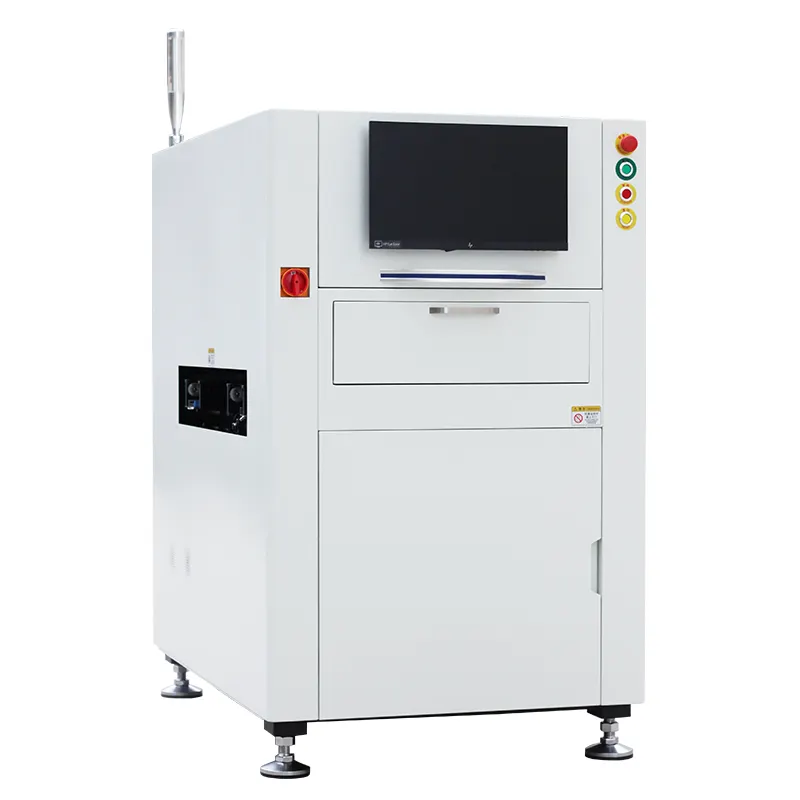
\includegraphics[width=0.38\columnwidth]{../../thesis-assets/01_aoi_machine/aoi.png}
\caption{SMT-line automatic AOI testing equipment. Source: HCT product documentation~\cite{hctaoi}.}
\label{fig:aoi_machine}
\end{figure}

\begin{table}[!ht]
\centering
\small
\caption{Representative Visible AOI Defect Categories (General Background)}
\label{tab:defect_taxonomy}
\begin{tabular}{p{0.22\columnwidth} p{0.28\columnwidth} p{0.40\columnwidth}}
\toprule
\textbf{Group} & \textbf{Event value} & \textbf{Description} \\
\midrule
Solder joint & \texttt{SOLDER\_BRIDGE} & Unintended connection between adjacent pads \\
Solder joint & \texttt{INSUFFICIENT\_SOLDER} & Solder volume below the acceptance requirement \\
Solder joint & \texttt{SOLDER\_BALL} & Excess solder particles on the board surface \\
Placement & \texttt{MISSING\_COMPONENT} & Component absent from its expected location \\
Placement & \texttt{MISALIGNMENT} & Component offset outside the allowed positional tolerance \\
Placement & \texttt{REVERSED\_POLARITY} & Polarized component placed in the wrong orientation \\
Lead & \texttt{BENT\_LEAD} & Lead deformation outside the accepted profile \\
Lead & \texttt{LIFTED\_LEAD} & Lead not in contact with its solder pad \\
\bottomrule
\end{tabular}

\vspace{0.3em}
\raggedright\footnotesize These categories illustrate the visible defects that AOI
addresses in general, organized against IPC-A-610H~\cite{ipc610h}. The detector
implemented in this work instead targets bare-board, fabrication-level defect
classes from the DsPCBSD+ dataset (Section~\ref{subsec:realmodel}); the
event schema itself stores \texttt{defect\_type} as a free-form string and is
agnostic to which taxonomy a detector emits.
\end{table}

%% TODO(human): Confirm with FUYU that the Holly training-deck defect grid may be reproduced in the public thesis.
\thesisfigure
{../../thesis-assets/01_aoi_machine/defects.png}
{Holly AOI defect-example grid from the training deck.}
{Representative AOI defect examples, including missing components, solder bridges, polarity errors, and lifted leads. Source: \textit{Holly AOI Training Guideline}, Shanghai Holly Electronics Co., Ltd. Reproduced subject to host-organization permission.\label{fig:defect_photos}}

\FloatBarrier

\subsection{Rule-Based and AI-Assisted AOI}

Classical AOI commonly applies reference-image comparison and engineered
thresholds, whereas learning-based methods infer decision boundaries from
training data. The latter can improve adaptability to complex visual variation,
but it also introduces operational questions about confidence, input shift, and
concept drift~\cite{ebayyeh2020aoi,ling2023pcb,gama2014drift}. These differences
motivate monitoring signals beyond a final pass/fail output.

Holly, documented by the training deck used in Figure~\ref{fig:aoi_machine}, is
the concrete rule-based example in this study~\cite{holly}; JUTZE~\cite{jutze}
and Flytake are AI-assisted examples, with Flytake documenting a multimodal
pipeline that combines YOLO/Ultralytics with optical character recognition
(OCR)~\cite{flytake}.

\begin{table}[!ht]
\centering
\small
\caption{Rule-Based and AI-Assisted AOI: Operational Comparison}
\label{tab:rule_vs_ai}
\begin{tabular}{p{0.22\columnwidth} p{0.31\columnwidth} p{0.35\columnwidth}}
\toprule
\textbf{Dimension} & \textbf{Rule-based AOI} & \textbf{AI-assisted AOI} \\
\midrule
Detection method & Reference comparison and explicit thresholds (e.g., Holly) & Learned features and decision boundaries (e.g., JUTZE; Flytake: YOLO/Ultralytics + OCR) \\
Adaptation & Rules and recipes are manually revised & Model or data pipeline is updated using representative data \\
False-call behavior & Often traceable to a threshold or recipe & Can change with confidence, calibration, or input distribution \\
Explainability & Decision rule is directly inspectable & Requires event evidence and operator-visible localization \\
Monitoring need & Recipe, image quality, throughput, and outcomes & The same signals plus confidence, drift, and model/runtime context \\
\bottomrule
\end{tabular}

\vspace{0.3em}
\raggedright\footnotesize Comparison synthesized from AOI survey literature~\cite{ebayyeh2020aoi,ling2023pcb}.
\end{table}

The review workstation provides a human-in-the-loop boundary: the AI proposes
an inspection result and overlay; an operator confirms or overrules it; and the
\texttt{operator\_review} state is retained with the defect record. This makes
human review part of the evidence chain rather than an unrecorded action, a
pattern consistent with feedback-centered ML engineering~\cite{amershi2019case}.
Figure~\ref{fig:state_review} models this review lifecycle as a UML state machine, in
which every defect record begins in \texttt{NONE} and is finalized as a confirmed or
overruled PASS/FAIL that is retained as evidence.
S04 then represents uncertainty under changed inputs, while S09 represents a
drift-like change whose evidence must remain visible over time.

\thesisfigure
{../../thesis-assets/00_generated_diagrams/hitl.png}
{Supply a diagram showing AI proposal, operator confirmation or override, and logged review outcome.}
{Human-in-the-loop AOI review: model output is presented to an operator, whose confirmation or override is retained as reviewable evidence.\label{fig:hitl_loop}}

\thesisfigure
{../../thesis-assets/00_generated_diagrams/state_review.png}
{Supply a UML state-machine diagram of the operator review lifecycle from NONE to the four confirmed/overruled outcomes.}
{Operator review lifecycle of a defect record (UML state machine), grounded in the \texttt{OperatorReview} states and the defect-review endpoint: every persisted defect begins in \texttt{NONE} and is finalized as a confirmed or overruled PASS/FAIL that is retained as evidence.\label{fig:state_review}}


\subsection{Related Work}

\subsubsection{Observability in Software Systems}
Observability is a core idea in distributed systems and production software~\cite{burns2016sre}.
Traditional monitoring emphasizes aggregate counters and infrastructure health,
while observability aims to make internal system behavior understandable through
logs, metrics, and traces. In AI systems, this distinction is important because
model-serving failures may appear even when CPU, memory, or network indicators
seem normal.

\subsubsection{Monitoring Stacks Based on Logs}
The Loki stack is a pragmatic logging solution for lightweight deployments~\cite{loki}.
Loki aggregates logs, Promtail ships them from services, and Grafana provides
queries, dashboards, and alert-friendly visualization~\cite{turnbull2018grafana}. Compared with heavyweight
full observability platforms, this stack is attractive for report-scale or
prototype environments because it is easy to deploy locally and integrates well
with structured JSON logs.

\subsubsection{ML and MLOps Monitoring}
Monitoring in machine learning systems usually covers several categories:
system health, inference latency, prediction distribution, data drift, model
versioning, and human feedback loops. Large MLOps platforms often include these
features~\cite{mlops}, but smaller projects frequently need a narrower and more direct
approach. For a local AOI workstation, the most relevant signals are event
volume, board throughput, failure frequency, confidence patterns, and per-event
latency.

This report is also informed by a broader software-engineering literature on ML
systems. Sculley et al.~\cite{sculley2015debt} argue that production ML systems accumulate system-level
technical debt through entanglement, hidden feedback loops, undeclared
consumers, and brittle interfaces rather than only through poor model
performance. Breck et al.~\cite{breck2017mltestscore} propose the ML Test Score as a production-readiness
rubric, emphasizing data validation, infrastructure testing, and monitoring
discipline around deployed models. Amershi et al.~\cite{amershi2019case} show, through an industrial
case study at Microsoft, that developing ML-enabled products requires a wider
process change than conventional software engineering, especially around data,
versioning, and integration. Shankar et al.~\cite{shankar2022observability, shankar2022interview} extend this discussion by arguing
that production ML pipelines require end-to-end observability because silent
failures often occur outside the model itself. These works strengthen the
motivation for a thesis that treats AOI inference as an operational system to
be monitored, not only a predictor to be benchmarked.

\subsubsection{Monitoring in Industrial Inspection}
Industrial inspection systems differ from generic web services because they are
tightly connected to physical workflows. Missing logs can make defect review
non-reproducible, while unstable latency can slow operator decisions. This
means monitoring must support both engineering needs and operational review.
This requirement mirrors the observability and MLOps principles discussed
above~\cite{burns2016sre, shankar2022observability}: trustworthy inspection
requires end-to-end traceability of each inference event.

\subsubsection{Comparison With Large-Scale Monitoring Platforms}
Large industrial AI systems often operate at a scale far beyond a bachelor
internship project, and it is useful to state this difference clearly. Netflix
reports that its Mantis platform has been in production since 2014 and
processes trillions of events and peta-bytes of data every day~\cite{mantis}. The same public
documentation describes use cases that analyze data from thousands of servers,
millions of interactions across dozens of microservices, and hundreds of
Cassandra and ElasticSearch clusters~\cite{mantisusecases}. In separate Netflix platform material,
the company also reports tens of thousands of running instances across its
deployment environment~\cite{netflixoss}.

This report does not attempt to replicate that scale. Instead, it adopts a
similar engineering principle at a much smaller scope: preserve structured raw
events, keep the monitoring pipeline queryable in near real time, and make it
possible to ask new operational questions without changing the application each
time a new anomaly is suspected.

It is also useful to compare the present design with specialized inference
servers such as NVIDIA Triton. Triton exposes a rich metrics surface including
request duration, queue duration, inference count, and execution count~\cite{tritonmetrics}. Those
capabilities are important in high-throughput GPU-serving environments. By
contrast, the AOI workstation in this report is optimized for local
deployability, defect traceability, and end-to-end observability of an AOI
review workflow rather than raw serving throughput. The tradeoff is deliberate:
FastAPI plus structured JSONL logging~\cite{fastapi} is easier to audit, easier to modify, and
better matched to a repository-scale case study than a full production-grade
inference platform.

\section{OBJECTIVES}

The objectives of this thesis are as follows:
\begin{itemize}
    \item Explain why inference monitoring matters in operational AI systems;
    \item Review observability practices relevant to ML services;
    \item Design a monitoring architecture suitable for a local AOI platform;
    \item Describe a concrete implementation grounded in the PCB AOI project;
    \item Propose experiments that simulate multiple runtime conditions; and
    \item Evaluate whether the system supports practical anomaly detection.
\end{itemize}


\section{MATERIALS AND METHODS}
\subsection{System Design}

\subsubsection{Monitoring Scope and Signal Selection}
Monitoring answers predefined operational questions, while observability also
supports investigation of behavior that was not anticipated when a dashboard
was created. This thesis therefore implements log-based monitoring with
observability-style ad-hoc LogQL investigation, rather than claiming a complete
three-signal observability platform~\cite{majors2022observability,sridharan2018distributed}.

\begin{table}[!ht]
\centering
\small
\caption{Logs, Metrics, and Traces in the Scope of This Thesis}
\label{tab:three_pillars}
\begin{tabular}{p{0.16\columnwidth} p{0.25\columnwidth} p{0.25\columnwidth} p{0.22\columnwidth}}
\toprule
\textbf{Signal} & \textbf{Primary unit} & \textbf{AOI use} & \textbf{Thesis scope} \\
\midrule
Logs & Structured event record & Board, component, result, confidence, latency, and review evidence & Implemented with JSONL, Promtail, and Loki \\
Metrics & Numeric time series & Rates, resource use, and service-level trends & Derived from logs; native exporters remain future work \\
Traces & Causally linked spans & Delay attribution across acquisition, inference, persistence, and review & Outside the single-service case-study scope \\
\bottomrule
\end{tabular}

\vspace{0.3em}
\raggedright\footnotesize Signal framing follows observability literature~\cite{majors2022observability,sridharan2018distributed}.
\end{table}

A log-centric design fits this bounded workflow because one record can preserve
both operational and AOI-domain context. Prometheus is designed around labeled
time series~\cite{prometheus}; it would complement the event evidence for native
resource metrics rather than replace it. OpenTelemetry provides a standard
framework for telemetry signals~\cite{opentelemetry}, but instrumenting traces
and metrics is outside the logs-only implementation scope and is retained as
future work.

\subsubsection{Log Aggregation Alternatives}
Loki indexes stream labels while retaining log content in chunks; Elasticsearch
uses an inverted indexing model, and OpenSearch provides a related open-source
search and analytics stack. Table~\ref{tab:log_aggregation} records the
architectural trade-off rather than a benchmark result.

\begin{table}[!ht]
\centering
\scriptsize
\caption{Architectural Comparison of Log Aggregation Alternatives}
\label{tab:log_aggregation}
\begin{tabular}{p{0.12\columnwidth} p{0.18\columnwidth} p{0.14\columnwidth} p{0.18\columnwidth} p{0.14\columnwidth} p{0.12\columnwidth}}
\toprule
\textbf{Stack} & \textbf{Indexing model} & \textbf{Query} & \textbf{Operational implication} & \textbf{Licensing} & \textbf{Dashboard} \\
\midrule
Loki & Labels index streams; content remains in chunks & LogQL & Bounded label set; direct fit with the existing Grafana stack & AGPL-3.0 & Grafana \\
Elasticsearch / ELK & Full-text inverted index & Query DSL / Lucene syntax & Rich document search with additional indexing work & Elastic License / SSPL for current default distribution & Kibana \\
OpenSearch & Full-text inverted index & Query DSL & Open-source search and analytics alternative with its own cluster services & Apache-2.0 & OpenSearch Dashboards \\
\bottomrule
\end{tabular}

\vspace{0.3em}
\raggedright\footnotesize Architecture and licensing descriptions use the primary project documentation~\cite{lokiarch,elasticsearchdocs,opensearchdocs}.
\end{table}

The selected Loki labels are categorical identifiers used by recurring
queries. Numeric values such as confidence and latency remain parsed JSON
fields. This follows Loki's guidance to avoid unbounded or high-cardinality
labels~\cite{lokilabels}; the actual active cardinality is left for the
measurement procedure in Section~4.1.5 and Table~\ref{tab:performance_resources}.
Grafana was retained because the
implemented system already provisions its Loki data source, dashboards, and
alerts as code; Kibana is the dashboard native to the Elasticsearch stack.

\subsubsection{Design Principles}
The proposed monitoring architecture follows five principles:
\begin{enumerate}
    \item Structured logs instead of free-form strings;
    \item Event schemas aligned with AOI domain entities;
    \item Separation between inference, persistence, and visualization;
    \item Local deployability for development and report demonstration; and
    \item Support for anomaly detection through simple, inspectable queries.
\end{enumerate}

\subsubsection{Architecture Overview}
The architecture begins with the AOI application, which emits inference events
as structured JSON entries. Each event may include a PCB identifier, component
identifier, inspection result, defect type, confidence score, latency, and
normalized overlay geometry. These logs are written to a file that Promtail
scrapes and forwards to Loki. Grafana then queries Loki to present operational
dashboards such as total events, recent failures, boards processed, and latency
trends.

In repository terms, the path is concrete rather than conceptual. A FastAPI API
accepts \texttt{POST /events} requests, writes event rows to JSONL, and stores
run metadata in SQLite. Promtail scrapes the shared JSON log volume,
extracts selected fields from each JSON object, and promotes a subset of those
fields to labels. Loki stores the resulting log streams, while Grafana provides
the dashboard and alerting surface. This design keeps the event source, log
transport, query model, and visual layer clearly separated. End to end, an event
becomes visible on the dashboards within a few seconds: Promtail tails the JSONL
files continuously and forwards them to Loki within roughly a second, and the
Grafana panels refresh on a 5-second interval. This 5-second refresh is the
practical bound on the ``near real time'' freshness referred to throughout this
report.

\subsubsection{Event Model}
The event schema is the core monitoring contract. An effective schema should
capture both model output and operational metadata. In the AOI case, the most
important fields are:
\begin{itemize}
    \item \texttt{timestamp} for temporal ordering;
    \item \texttt{pcb\_id} for board-level grouping;
    \item \texttt{component\_id} for defect localization;
    \item \texttt{inspection\_result} for pass/fail state;
    \item \texttt{defect\_type} for defect categorization;
    \item \texttt{confidence\_score} for prediction strength;
    \item \texttt{inference\_latency\_ms} for performance monitoring; and
    \item overlay coordinates for frontend review traceability.
\end{itemize}

This field selection is intentionally narrower than a full cloud MLOps schema.
The goal is to preserve the signals most relevant to AOI operation while
keeping queries simple. In the Promtail pipeline, \texttt{pcb\_id},
\texttt{component\_id}, \texttt{inspection\_result}, and
\texttt{defect\_type} are promoted to labels because they are frequently used
for filtering and grouping. By contrast, \texttt{confidence\_score} and
\texttt{inference\_latency\_ms} remain JSON values that are parsed on demand
through LogQL \texttt{| json | unwrap ...} expressions. This reduces label
cardinality while preserving numeric analysis.
At the prototype scale of 131 boards, retaining \texttt{pcb\_id} as a label is
a deliberate choice for query ergonomics; in production, it should instead be
parsed on demand as a JSON field like confidence and latency.

\begin{figure}[!ht]
\centering
\small
\fbox{\begin{minipage}{0.94\columnwidth}
\centering
\textbf{InferenceEvent monitoring contract}\\[0.5em]
\begin{tabular}{p{0.30\columnwidth} p{0.27\columnwidth} p{0.29\columnwidth}}
\toprule
\textbf{Event fields} & \textbf{Promoted Loki labels} & \textbf{Parsed JSON values} \\
\midrule
\texttt{timestamp} & \texttt{pcb\_id} & \texttt{confidence\_score} \\
\texttt{pcb\_id} & \texttt{component\_id} & \texttt{inference\_latency\_ms} \\
\texttt{component\_id} & \texttt{inspection\_result} & overlay coordinates and shape \\
\texttt{inspection\_result} & \texttt{defect\_type} & other event fields parsed on demand \\
\texttt{defect\_type} & & \\
\texttt{confidence\_score} & & \\
\texttt{inference\_latency\_ms} & & \\
overlay fields & & \\
\bottomrule
\end{tabular}
\end{minipage}}
\caption{Mapping from the \texttt{InferenceEvent} schema to Loki. Frequently filtered identifiers become labels, while numeric and overlay values remain structured JSON fields; this supports reproducible LogQL analysis without promoting every field to a high-cardinality label.}
\label{fig:event_label_mapping}
\end{figure}

\subsubsection{Dashboard Logic}
The dashboard is designed around operational questions:
\begin{itemize}
    \item How many events arrived in the last five minutes?
    \item How many recent detections were failures?
    \item How many boards were processed in a recent time window?
    \item Is inference latency stable or increasing?
\end{itemize}
These questions map directly to Loki queries and make the dashboard useful for
both live monitoring and retrospective investigation.

\subsubsection{Anomaly Types}
The design groups anomalies by the operational signal that changes: traffic
volume, prediction outcomes, latency, confidence, or domain identifiers such as
\texttt{pcb\_id} and \texttt{defect\_type}. This compact taxonomy determines
which fields must be logged and which dashboard queries must be supported; the
specific test scenarios are defined in Section~3.3 and summarized in
Table~\ref{tab:scenario_suite}.

\subsubsection{Why This Design Pattern Was Chosen}
The monitoring architecture follows a log-centric MLOps pattern for four
practical reasons.
\begin{enumerate}
    \item \textbf{Low integration cost.} A FastAPI service can emit structured
    JSON without introducing a specialized model server or a metric exporter at
    the first stage of the project.
    \item \textbf{High diagnostic value.} A single event record can carry both
    operational fields such as latency and AOI-specific fields such as
    \texttt{pcb\_id} and \texttt{defect\_type}. This is harder to capture in
    aggregate metrics alone.
    \item \textbf{Observability as code.} Promtail parsing rules, Grafana
    dashboards, and alert thresholds are provisioned from version-controlled
    files, which makes the monitoring behavior reproducible.
    \item \textbf{Fit to scope.} The thesis question is whether anomalies in an
    AOI inference service become visible and actionable. It is not whether the
    repository can outperform industrial serving platforms on throughput.
\end{enumerate}

The main alternative would be a production inference stack centered on systems
such as Triton, KServe, or a larger stream-processing platform. Those
architectures are stronger when dynamic batching, GPU multiplexing, autoscaling,
or multi-tenant serving are the central problem. In this project, however, the
critical problem is explainable monitoring around a bounded AOI workflow. The
chosen pattern therefore prioritizes interpretability over maximum serving
complexity.

\subsubsection{MLOps and Observability-as-Code Patterns}
Although the implementation is lightweight, it still follows several recognizably
MLOps-oriented patterns:
\begin{itemize}
    \item \textbf{Schema as contract:} the event structure standardizes what an
    inference result must contain before it enters the monitoring stack.
    \item \textbf{Logs as canonical evidence:} every experiment ultimately
    becomes a sequence of JSONL records that can be replayed, queried, and
    audited.
    \item \textbf{Infrastructure as code:} alert rules and scrape pipelines are
    defined in YAML rather than configured manually in a UI.
    \item \textbf{Experiment harness separation:} scenario generation,
    sequential execution, and report extraction are implemented as separate
    modules rather than one ad hoc script.
\end{itemize}

% Previous ASCII version retained for traceability:
% \begin{figure}[!ht]
% \centering
% \fbox{\begin{minipage}{0.94\columnwidth}
% \centering
% \textbf{Event source} \textrightarrow{} \texttt{POST /events}
% \textrightarrow{} \textbf{FastAPI validation}\\[0.6em]
% \textrightarrow{} \textbf{SQLite review state + JSONL evidence}
% \textrightarrow{} \textbf{Promtail}\\[0.6em]
% \textrightarrow{} \textbf{Loki}
% \textrightarrow{} \textbf{Grafana dashboards / alerts}\\[0.6em]
% \textrightarrow{} \textbf{LogQL queries / generated report}
% \end{minipage}}
% \caption{Implemented repository-aligned observability architecture. Synthetic or future real inference events traverse the same FastAPI, persistence, log-shipping, Loki, Grafana, and report path; no autonomous agent or retraining stage is part of the implemented system.}
% \label{fig:implemented_architecture}
% \end{figure}
\thesisfigure
{../../thesis-assets/00_generated_diagrams/aoi_inference_workflow.png}
{Supply the repository-aligned architecture diagram from event source through FastAPI, SQLite/JSONL, Promtail, Loki, and Grafana.}
{Implemented repository-aligned observability architecture. Synthetic or future real inference events traverse the same FastAPI, persistence, log-shipping, Loki, Grafana, and report path; no autonomous agent or retraining stage is part of the implemented system.\label{fig:implemented_architecture}}

\thesisfigure
{../../thesis-assets/00_generated_diagrams/use_case.png}
{Supply a UML use-case diagram with the Operator, ML/Platform Engineer, and Inference Service actors.}
{Use-case diagram (UML): the Operator drives run creation, scan upload, setup, and defect review; the Inference Service runs the model and emits events; the ML/Platform Engineer monitors dashboards and investigates anomalies.\label{fig:use_case}}

\thesisfigure
{../../thesis-assets/00_generated_diagrams/class_diagram.png}
{Supply a UML class diagram of the backend services (DatabaseManager, SetupService, VisionService, LogManager) and the schema types.}
{Backend class diagram (UML): the FastAPI routes drive \texttt{DatabaseManager}, which delegates setup to \texttt{SetupService} and detection to \texttt{VisionService}; \texttt{LogManager} appends each event to JSONL, and the inference runner produces \texttt{InferenceEvent}s carrying \texttt{InspectionResult} and \texttt{OperatorReview}.\label{fig:class_diagram}}


\subsection{Case Study Implementation}

\subsubsection{Repository-Aligned AOI Platform}
The case study implementation is based on the current AOI repository. The
backend is implemented in Python with FastAPI and exposes routes for health,
runs, and event ingestion. Figure~\ref{fig:use_case} maps the actors---the operator,
the ML/platform engineer, and the inference service---to these capabilities, and
Figure~\ref{fig:class_diagram} details the backend service classes
(\texttt{DatabaseManager}, \texttt{SetupService}, \texttt{VisionService},
\texttt{LogManager}) and the schema types that implement them. The frontend is a
React workstation for PCB review,
including run navigation, image viewing, overlay display, and operator review
controls. SQLite is used for local persistence, and JSONL is used for event log
output.

\subsubsection{Implemented Monitoring Components}
The implementation contains the following concrete monitoring-relevant modules:
\begin{itemize}
    \item a Schema layer defining \texttt{InferenceEvent} and inspection states;
    \item a Log manager that appends JSON records to persistent log files;
    \item a Mock inference generator for controlled event simulation;
    \item a Docker Compose stack containing Loki, Promtail, and Grafana; and
    \item a Provisioned Grafana dashboard for AOI event inspection.
\end{itemize}

Two implementation details are especially important. First, the Promtail
configuration parses JSON and promotes domain identifiers to labels. This is
what makes queries such as \texttt{\{job="aoi-inference",
pcb\_id=~"PCB-DEAD-.*"\}} possible without full-text search. Second, the alert
rules are provisioned as code in Grafana, with three explicit threshold
policies: fail rate \(> 0.60\), average latency \(> 500\) ms, and average
confidence \(< 0.60\). Each rule follows the same pattern: a Loki range query,
a reduce stage, and a threshold stage.

These prototype thresholds are derived from the S01 baseline in
Table~\ref{tab:scenario_quantitative_profile}: the 0.60 fail-rate threshold is
well above the baseline's roughly 10\% fail rate, 500\,ms is above the normal
CPU-inference latency (on the order of 100--200\,ms), and the 0.60 confidence
bound is below the high average confidence of clean-board operation. Each
threshold therefore lies outside the baseline with headroom; calibration against
representative production data remains required as stated in
Section~\ref{sec:future_work}.

\subsubsection{Event Flow in the AOI Service}
The service receives or generates inference-like outputs and converts them into
structured events. A typical event includes board identity, component identity,
inspection result, defect type, confidence score, latency, and optional defect
overlay coordinates. The backend can then persist the event and expose related
data to the review workstation. This creates a direct path from AI output to
human inspection and to observability tooling.

\subsubsection{Why the AOI Project is a Good Monitoring Case}
The AOI project is appropriate for monitoring research because it combines
image processing, event logging, persistence, operator review, and dashboarding
within a single system. Its controlled event generator makes the platform
suitable for reproducible failure-scenario experiments and report
demonstration without requiring a fully deployed production model.

\subsubsection{Code Pattern: Event Construction and Safe Emission}
The experiment harness avoids raw dictionary duplication by centralizing event
construction in the shared scenario helper module. The helper function
\texttt{make\_event(...)} clamps confidence to the API's accepted range,
prevents negative latency values, and only emits overlay geometry when the
inspection result is \texttt{FAIL}. This is a useful pattern because it keeps
scenario scripts focused on behavior rather than payload plumbing.

\begin{lstlisting}[language=Python,caption={Core event-construction pattern in the shared scenario helper.},label={lst:make_event}]
def make_event(...):
    confidence_score = max(0.0, min(1.0, confidence_score))
    inference_latency_ms = max(0, inference_latency_ms)
    event = {
        "pcb_id": pcb_id,
        "component_id": component_id,
        "inspection_result": inspection_result,
        "defect_type": defect_type,
        "confidence_score": confidence_score,
        "inference_latency_ms": inference_latency_ms,
        "overlay_shape": "rect" if inspection_result == "FAIL" else None,
    }
    return {k: v for k, v in event.items() if v is not None}
\end{lstlisting}

The batch sender in the same module provides a second useful pattern: scenario
scripts prepare batches only, while HTTP posting, timing, and error collection
are handled centrally. This design reduces code duplication and guarantees that
all nine scenarios are measured in the same way.

\begin{table}[!ht]
\centering
\caption{Case Study Components and Monitoring Roles}
\label{tab:case_components}
\begin{tabular}{p{0.22\columnwidth} p{0.23\columnwidth} p{0.42\columnwidth}}
\toprule
\textbf{Layer} & \textbf{Component} & \textbf{Monitoring Role} \\
\midrule
API backend & FastAPI service & Accepts events, exposes health, supports run review \\
Schema & \texttt{InferenceEvent} & Defines structured monitoring payload \\
Logging & JSONL log manager & Persists machine-readable events \\
Transport & Promtail & Ships logs to aggregation layer \\
Storage & Loki & Indexes and queries log streams \\
Visualization & Grafana dashboard & Shows event volume, failures, boards, latency \\
Frontend & React workstation & Uses event data for review traceability \\
\bottomrule
\end{tabular}
\end{table}

\thesisfigure
{../../assets/readme/review-workspace.png}
{AOI review workstation showing the uploaded PCB scan, run history, filters, defect queue, and review canvas.}
{Implemented AOI review workstation with a representative PCB scan uploaded through the live setup workflow. The run browser and filters appear at left, while the defect queue and PCB review canvas provide the operator-facing inspection surface.}

\subsubsection{REST API Design}
The backend exposes resource-oriented HTTP endpoints and publishes its generated
OpenAPI description through FastAPI. The event-ingestion contract is implemented
by \texttt{POST /events}; the run and
review routes connect the same accepted events to the operator workstation. This
separation follows REST's resource-oriented interface constraints~\cite{fielding2000rest}
while retaining Pydantic validation and generated API documentation~\cite{fastapi}.

\begin{table}[!ht]
\centering
\small
\caption{Principal REST API Endpoints Used by the Monitoring and Review Workflow}
\label{tab:api_endpoints}
\begin{tabular}{p{0.13\columnwidth} p{0.34\columnwidth} p{0.10\columnwidth} p{0.31\columnwidth}}
\toprule
\textbf{Method} & \textbf{Path} & \textbf{Success} & \textbf{Purpose} \\
\midrule
GET & \texttt{/health} & 200 & Check API availability \\
POST & \texttt{/events} & 202 & Validate, log, and persist one event or an event batch \\
POST & \texttt{/runs} & 201 & Create an inspection run \\
GET & \texttt{/runs} & 200 & List runs with optional filters \\
GET & \texttt{/runs/\{run\_id\}} & 200 & Retrieve a run and its defect records \\
GET & \texttt{/runs/\{run\_id\}/defects} & 200 & Retrieve filtered defects for one run \\
POST & \texttt{/runs/\{run\_id\}/images} & 201 & Attach the full-board image to a run \\
PATCH & \texttt{/runs/\{run\_id\}/}\newline\texttt{defects/\{defect\_id\}/review} & 200 & Store an operator review decision \\
\bottomrule
\end{tabular}
\end{table}

The complete request-to-dashboard sequence is shown in
Figure~\ref{fig:experiment_workflow}.

\subsubsection{Event and JSON Schema}
The implementation has two explicit schema layers. The Pydantic
\texttt{EventIn} model validates the HTTP payload and converts it to the domain
\texttt{InferenceEvent} dataclass. Listing~\ref{lst:event_in} reproduces the
actual inbound request-field declarations; naming this model \texttt{EventIn}
preserves the real class boundary rather than conflating the API and domain
types.

\begin{lstlisting}[language=Python,caption={Pydantic event request model used by the implemented API.},label={lst:event_in}]
class EventIn(BaseModel):
    model_config = ConfigDict(extra="forbid")

    timestamp: str | None = None
    pcb_id: str
    component_id: str
    inspection_result: InspectionResult
    defect_type: str
    confidence_score: float = Field(ge=0.0, le=1.0)
    inference_latency_ms: int = Field(ge=0)
    run_image_index: int | None = Field(default=None, ge=0)
    overlay_x: float | None = Field(default=None, ge=0.0, le=1.0)
    overlay_y: float | None = Field(default=None, ge=0.0, le=1.0)
    overlay_width: float | None = Field(default=None, ge=0.0, le=1.0)
    overlay_height: float | None = Field(default=None, ge=0.0, le=1.0)
    overlay_shape: str | None = None
    operator_review: OperatorReview = OperatorReview.NONE
\end{lstlisting}

The model forbids unknown fields; requires non-empty board, component, and
defect strings; constrains confidence and normalized overlay values to
\([0,1]\); requires non-negative latency and image indices; and validates an
optional timestamp as ISO~8601. Invalid JSON is returned as HTTP 400, while
schema violations are returned as HTTP 422. Accepted input is converted through
\texttt{to\_domain()} before persistence and JSONL emission.

\subsubsection{Database Design}
SQLite provides local relational persistence for the single-workstation case
study~\cite{gaffney2022sqlite}. The implemented schema makes
\texttt{inspection\_runs} the parent record; \texttt{defect\_logs} and
\texttt{run\_images} reference a run, while \texttt{model\_fovs} stores reusable
normalized regions associated with a model name. Defect rows retain confidence,
latency, result, overlay geometry, and \texttt{operator\_review}, which connects
model output to the human-in-the-loop evidence described in
Figure~\ref{fig:hitl_loop}.

\begin{table}[!ht]
\centering
\small
\caption{Implemented SQLite Entities and Relationships}
\label{tab:database_entities}
\begin{tabular}{p{0.24\columnwidth} p{0.29\columnwidth} p{0.35\columnwidth}}
\toprule
\textbf{Entity} & \textbf{Key relationship} & \textbf{Monitoring or review role} \\
\midrule
\texttt{inspection\_runs} & Primary key \texttt{id} & Board identity, timestamp, model, setup state, and aggregate status \\
\texttt{defect\_logs} & Foreign key \texttt{run\_id} & Component result, defect, confidence, latency, overlay, and review state \\
\texttt{run\_images} & Foreign key \texttt{run\_id} & Image path, dimensions, role, and display order \\
\texttt{model\_fovs} & Associated by \texttt{model\_name} & Reusable normalized component fields of view \\
\bottomrule
\end{tabular}
\end{table}

\thesisfigure
{../../thesis-assets/00_generated_diagrams/er_diagram.png}
{Supply an ER diagram for \texttt{inspection\_runs}, \texttt{defect\_logs}, \texttt{run\_images}, and \texttt{model\_fovs}.}
{Implemented SQLite relationships supporting \texttt{inspection\_runs}, defect-level results, images, model fields of view, and operator review.\label{fig:database_er}}

\subsubsection{Frontend Architecture}
The React workstation requests run and defect resources from the API, maintains
the selected run and defect in UI state, and renders normalized overlay geometry
over the selected board image. The run rail and filters provide navigation; the
canvas provides spatial context; and the inspector sends review updates back to
the API. React is used as the component-based view layer~\cite{reactdocs}; the
backend remains the persistence boundary rather than duplicating review state
inside the browser.

\subsubsection{Deployment}
Docker Compose defines the deployable service topology: \texttt{aoi-app} and
\texttt{aoi-web} provide the application, while Promtail, Loki, and Grafana
provide log transport, storage, querying, and visualization. The named
\texttt{aoi-logs} volume is mounted read-write by the API and read-only by
Promtail; \texttt{aoi-data} retains local application data. Compose therefore
keeps service configuration reproducible and isolates dependencies in
containers~\cite{merkel2014docker,bernstein2014containers}.

\thesisfigure
{../../thesis-assets/00_generated_diagrams/docker.png}
{Supply a topology diagram showing aoi-web, aoi-app, aoi-logs, aoi-data, Promtail, Loki, and Grafana.}
{Docker Compose deployment topology and the shared log path from the API container through Promtail to Loki and Grafana.\label{fig:docker_topology}}


\subsection{Defect Detection Model and Real Inference Integration}\label{subsec:realmodel}

\subsubsection{Dataset and Model}
To move the case study from synthetically generated events toward genuine model
inference, a real defect detector was trained and connected to the same ingestion
path. The detector targets PCB fabrication and trace defects using the public
DsPCBSD+ dataset~\cite{dspcbsd} (Creative Commons BY~4.0), which provides
10{,}259 annotated images across nine defect classes: short, spur, spurious
copper, open, mouse-bite, hole-breakout, conductor scratch, conductor foreign
object, and base-material foreign object. A deterministic, seeded conversion
script normalizes the download into a YOLOv8 layout with a 7{,}388 / 2{,}051 /
820 train/validation/test split, so the dataset preparation is reproducible.

A YOLOv8s detector~\cite{ultralytics} was fine-tuned on this dataset (a baseline
configuration and a channel-attention variant), and a deliberately under-trained
early checkpoint was retained to emulate model degradation. Training was performed
on a Colab GPU and the exported weights were placed back into the repository;
inference itself runs comfortably on CPU at the prototype scale.

\subsubsection{Inference Integration}
A real inference runner loads the trained weights, runs prediction on a PCB
image, and converts each detection into the same \texttt{InferenceEvent} schema
used throughout the system: the detected class becomes the \texttt{defect\_type},
the detector score becomes \texttt{confidence\_score}, the measured wall-clock
time becomes \texttt{inference\_latency\_ms}, and the normalized bounding box
becomes the overlay. An image with no detection above threshold yields a single
\texttt{PASS}/\texttt{NO\_DEFECT} event, while an unreadable or corrupt scan
yields a board-level \texttt{BOARD\_FAILURE} event rather than crashing the batch.
These events are POSTed to the identical \texttt{/events} endpoint used by the
synthetic generator, so real model output traverses the same FastAPI, SQLite and
JSONL persistence, Promtail, Loki, and Grafana path
(Figure~\ref{fig:implemented_architecture}) with no downstream change. The
inference runner also writes a \texttt{model\_version} label with each event,
making model identity a first-class, queryable monitoring dimension.

This design preserves the monitoring focus of the thesis while removing the main
authenticity limitation of the earlier mock-only pipeline: the signals observed
in Grafana---confidence, latency, defect type, and fail rate---are now produced by
a real convolutional detector rather than by hand-written values.

\subsubsection{Real-Image Corpus and Scenario Coverage}
A small evaluation corpus is derived from the held-out test split: defect-free
crops (regions of real boards carrying no annotation, used as the
\texttt{PASS}-dominated baseline), defective boards, blurred/noisy/downscaled
copies of defective boards, and intentionally corrupt files. Driven from this
corpus, eight of the nine anomaly scenarios are produced by real inference; only
the latency profile of S03 remains injected, because a genuine latency spike
cannot be summoned on demand. Model degradation (S09) is realized by running the
same defective boards first through the trained baseline and then through the
under-trained checkpoint, each tagged with its own \texttt{model\_version}.

\subsection{Experiments}

\subsubsection{Experimental Goal}
The experimental objective is to determine whether the monitoring stack can
differentiate between normal and abnormal inference behavior. The experiments are
driven by a real trained defect detector (Section~\ref{subsec:realmodel}), with controlled injection
retained only for conditions---such as a latency spike---that cannot be triggered
on demand. This staged approach is appropriate for a bachelor internship because
it allows repeated, explainable, and low-risk validation of monitoring behavior
before full factory deployment.

\subsubsection{Experiment Design}
The anomaly-testing plan defines a sequence of controlled scenarios that drive a
target operational state by choosing what the trained detector is run on, rather
than by hand-writing event values. Each scenario emphasizes one monitored signal,
such as fail rate, latency, confidence, defect mix, or temporal stability, while
keeping the rest of the pipeline intact: most scenarios obtain that signal from
real inference over a curated set of boards (defect-free crops, defective boards,
degraded copies, or corrupt files), and only the latency profile is injected
directly because a genuine latency spike cannot be summoned on demand. This makes
it possible to observe whether Grafana panels, Loki queries, and alert thresholds
respond as expected.

\subsubsection{End-to-End Experimental Workflow}
Every scenario uses the same end-to-end ingestion and monitoring path as the
AOI service. A scenario module runs the trained detector over a set of real PCB
images, converts each detection into an inspection event, and sends the batch as
an HTTP \texttt{POST} request to the FastAPI \texttt{/events} endpoint. The API validates field names, enumerated inspection
results, confidence bounds, non-negative latency, and required identifiers
before converting the request into domain events. Accepted events are appended
to the structured JSONL log, while the accepted batch is also persisted in
SQLite for run and defect review.

Promtail reads the JSONL file from the shared log volume, parses each line, and
promotes \texttt{pcb\_id}, \texttt{component\_id},
\texttt{inspection\_result}, \texttt{defect\_type}, and \texttt{model\_version} to
Loki labels. Loki
stores the resulting streams and makes both label filters and parsed numeric
fields available to LogQL. Grafana then queries those streams for dashboard
panels and provisioned alerts. Finally, a Loki-backed reporting step queries
the Loki HTTP API and produces a Markdown report, so the reported evidence is
derived from the same records that passed through the complete monitoring
stack rather than directly from the scenario runner.

% Previous ASCII version retained for traceability:
% \begin{figure}[!ht]
% \centering
% \fbox{\begin{minipage}{0.94\columnwidth}
% \centering
% \textbf{1 Scenario generator} \textrightarrow{} \textbf{2 Synthetic AOI event}
% \textrightarrow{} \textbf{3 HTTP \texttt{POST /events}}\\[0.6em]
% \textrightarrow{} \textbf{4 FastAPI schema validation}
% \textrightarrow{} \textbf{5a SQLite persistence + 5b JSONL append}\\[0.6em]
% \textrightarrow{} \textbf{6 Promtail scrape}
% \textrightarrow{} \textbf{7 Loki storage / query}\\[0.6em]
% \textrightarrow{} \textbf{8 Grafana dashboard / alert}
% \textrightarrow{} \textbf{9 Loki-backed report}
% \end{minipage}}
% \caption{Runtime lifecycle of one experiment event through the complete monitoring stack.}
% \label{fig:experiment_workflow}
% \end{figure}
\thesisfigure
{../../thesis-assets/00_generated_diagrams/Sequence_Event.png}
{Supply the experiment workflow from scenario generation to the Loki-backed report.}
{Runtime lifecycle of one experiment event through the API, validation, persistence, shipping, storage, visualization, and reporting stages.\label{fig:experiment_workflow}}

\subsubsection{Controlled Anomaly Injection Methodology}
The experimental control is the event-processing pipeline itself: endpoint,
schema, persistence code, Promtail configuration, Loki storage, and Grafana
queries are unchanged between scenarios. S02--S06 each elicit one monitored signal
or grouping dimension from real inference over a chosen set of boards (with only
S03's latency injected on top of real predictions); S07--S09 vary the temporal
pattern to test recovery, intermittent bursts, and a real model-version
regression. Scenario-specific \texttt{pcb\_id} prefixes allow the resulting
streams to be isolated without changing the ingestion path.

\textbf{Fail-rate anomaly (S02).}
S02 runs the detector over a batch of real defective boards, which yields a
\texttt{FAIL}-dominated stream at normal latency and real model confidence.
This represents a sudden process fault such as a bad material reel or placement
problem. The expected response is a dominant \texttt{FAIL} series and a
fail-rate alert above 0.60; the observed dashboard separation and Loki counts
confirm that the pipeline preserves and aggregates the changed outcome rate.

\textbf{Latency anomaly (S03).}
S03 keeps the detector's real predictions but overrides
\texttt{inference\_latency\_ms}, escalating it from a normal baseline toward a
2000\,ms plateau. This is realistic for resource contention, accelerator
starvation, or a degraded model runtime, and is the one signal injected directly
because a genuine spike cannot be summoned on demand. The latency panel and threshold alert rise while events continue to
arrive, validating that service performance can be monitored independently of
prediction outcome.

\textbf{Confidence anomaly (S04).}
S04 runs the detector over blurred, noisy, and downscaled copies of defective
boards, which lowers the detector's own \texttt{confidence\_score} and causes some
defects to be missed. Such degraded input is realistic when image conditions
differ from the data on which the detector was trained. The expected response is
a lower average-confidence panel and matching low-confidence LogQL results, which
validates numeric-field parsing and querying through Loki on genuine model
output.

\textbf{Defect-concentration anomaly (S05).}
S05 selects real detections of a single dominant defect class (\texttt{SPUR} in
the executed run) so that one \texttt{defect\_type} dominates failing events. This
models a systematic fabrication problem that repeats across boards. Grafana should show one defect series dominating and a
label-filtered Loki query should retrieve the same population; the observed
breakdown demonstrates that categorical fault patterns remain distinguishable
after ingestion.

\textbf{Board-grouping anomaly (S06).}
S06 feeds unreadable or corrupt scans that the detector cannot process; these
emit board-level \texttt{BOARD\_FAILURE} events under \texttt{PCB-DEAD-*}
identifiers, surrounded by normal boards. This represents a board-level failure
that may be obscured in an aggregate line-wide rate. Grouping or filtering by
\texttt{pcb\_id} is expected to isolate the affected boards, and the observed
per-board query result validates traceability from an overview signal to the
individual PCB.

\textbf{Recovery lifecycle (S07).}
S07 sequences a fault phase (real defective boards) into a recovery phase (real
clean boards), moving from a high-failure to a low-failure state. This is
realistic after an operator correction or service remediation and tests whether
monitoring represents resolution as well as onset. The dashboard's crossover toward
healthy values, together with alert recovery behavior, validates preservation
of the complete fault lifecycle.

\textbf{Intermittent bursts (S08).}
S08 places real defective-board bursts at positions 5, 11, and 17 within
otherwise clean-board traffic. Intermittent contact, vibration, or upstream
handling faults can create this non-continuous pattern, which broad averages
may dilute. The expected response is a set of narrow time-series spikes and
matching short-window Loki results; their observed visibility demonstrates the
value of retaining event-level history.

\textbf{Gradual degradation (S09).}
S09 runs the same real defective boards first through the trained baseline and
then through a deliberately under-trained checkpoint, each tagged with its own
\texttt{model\_version}. On identical boards the under-trained model detects far
fewer defects, producing a real model-version regression rather than a hand-set
decline. The expected monitoring response is a sharp drop in detected defects per
\texttt{model\_version}, and the observed shape validates that a model regression
remains visible and queryable after aggregation.

\subsubsection{Experiment Harness: Build, Run, and Report}
The implemented experiment lifecycle separates generation, execution, and
reporting into three stages, summarized below.

\textbf{Build stage.} Individual scenario modules, such as those for S02 and S03,
build their batches by running the detector over a corpus pool through a shared
\texttt{real\_model\_batches} helper. For example, S02 runs the model over real
defective boards, while S03 keeps the real predictions but raises
\texttt{inference\_latency\_ms} toward a 2000\,ms plateau. This is how the test
scenes are built.

\textbf{Run stage.} The experiment runner maps scenario IDs
S01--S09 to their generators and executes them sequentially. A 15-second pause
is inserted between scenarios so that Grafana time-series panels show visually
separated anomaly windows instead of one merged stream.

\begin{lstlisting}[language=Python,caption={Scenario orchestration pattern in the experiment runner.},label={lst:runner}]
ALL_SCENARIOS = {"S01": s01_normal_baseline, ..., "S09": s09_model_degradation}
INTER_SCENARIO_PAUSE_SECONDS = 15

for idx, scenario_id in enumerate(targets):
    module = ALL_SCENARIOS[scenario_id]
    result = module.run(endpoint=endpoint)
    results.append(result)
    if idx < len(targets) - 1:
        time.sleep(INTER_SCENARIO_PAUSE_SECONDS)
\end{lstlisting}

\textbf{Report stage.} After execution, the reporting step queries
Loki directly through its HTTP API, counts matching log entries over a lookback
window, and produces the final evaluation report summarized in
Section~4.1.6. This closes the loop from test generation to runtime evidence
and reported results.

\begin{lstlisting}[language=Python,caption={Loki-backed report generation pattern.},label={lst:report}]
total_events = count_logs('{job="aoi-inference"}', lookback_minutes)
total_fails = count_logs('{job="aoi-inference", inspection_result="FAIL"}',
                         lookback_minutes)
fail_rate = (total_fails / total_events * 100) if total_events else 0
output_path.write_text("\n".join(lines))
\end{lstlisting}

This three-part split is a deliberate design choice that makes the experiment
suite reproducible and easier to extend. Listings~\ref{lst:runner} and
\ref{lst:report} make the generation, execution, and result-computation steps
explicit within this thesis.

\subsubsection{Reproducibility Procedure}
An evaluator can reproduce the experiment from the repository root with the
following repository-defined commands:

\begin{lstlisting}[language=bash,caption={Commands for reproducing the anomaly experiment suite.},label={lst:reproduce}]
docker compose up -d --build
python3 -m experiments.runner
python3 -m experiments.report --output docs/experiments/anomaly_results.md
\end{lstlisting}

The first command starts the FastAPI service, Promtail, Loki, and Grafana from
the repository's Compose configuration. The second command executes S01--S09;
selected scenarios can instead be chosen with the runner's
\texttt{--scenarios} option. During or after execution, the evaluator can open
the local Grafana service on port 3000 using the repository defaults
(\texttt{admin}/\texttt{admin}) and inspect the provisioned AOI dashboard or
run the scenario queries in Explore. The final command reads the preceding
120 minutes from Loki and writes the retained report to the output path shown
in Listing~\ref{lst:reproduce}. The stack can be stopped with
\texttt{docker compose down}.

\subsubsection{Scenario Set}
The experiment suite contains one baseline scenario and multiple anomaly
scenarios. The baseline establishes normal operating behavior, while the other
scenarios test the system's ability to detect spikes, drifts, and recovery.

\begin{table}[!ht]
\centering
\caption{Anomaly Testing Scenarios}
\label{tab:scenario_suite}
\begin{tabular}{p{0.11\columnwidth} p{0.28\columnwidth} p{0.46\columnwidth}}
\toprule
\textbf{ID} & \textbf{Scenario} & \textbf{Main Monitoring Purpose} \\
\midrule
S01 & Normal baseline & establish healthy reference traffic and baseline latency \\
S02 & High defect rate spike & detect sudden fail-rate anomaly \\
S03 & Latency spike & detect severe inference slowdown \\
S04 & Low confidence storm & detect model uncertainty or out-of-distribution behavior \\
S05 & Single defect-type flood & isolate systematic failure patterns by defect label \\
S06 & Board-level failure & isolate catastrophic failures affecting specific boards \\
S07 & System recovery & verify anomaly resolution and alert recovery \\
S08 & Intermittent faults & detect short bursts that may be hidden in aggregates \\
S09 & Gradual model degradation & detect long-horizon confidence decline and fail-rate growth \\
\bottomrule
\end{tabular}
\end{table}

\begin{table}[!ht]
\centering
\small
\caption{Repository-Scale Design Decisions and Considered Alternatives}
\label{tab:design_decisions}
\begin{tabular}{p{0.15\columnwidth} p{0.17\columnwidth} p{0.43\columnwidth} p{0.15\columnwidth}}
\toprule
\textbf{Design choice} & \textbf{Alternative} & \textbf{Reason chosen for this case study} & \textbf{Citation} \\
\midrule
FastAPI & Flask & Type validation, generated API documentation, and alignment with the Python inference ecosystem & \cite{fastapi,techempower} \\
Loki & Elasticsearch / ELK & Label-indexed local log aggregation and direct Grafana integration & \cite{lokiarch} \\
JSONL & Plain-text logs & Structured, line-oriented records that are parseable and replayable & \cite{twelvefactor} \\
SQLite & PostgreSQL & Low-setup local persistence appropriate for a single-workstation case study & \cite{gaffney2022sqlite} \\
LogQL & Manual grep & Reproducible filters, aggregations, dashboards, and alert queries & \cite{loki} \\
React & Vue / Angular & Component-based workstation UI integrated with the repository's existing frontend & \cite{reactdocs} \\
Docker Compose & Manual service setup & Reproducible local topology, versions, volumes, and service dependencies & \cite{merkel2014docker,bernstein2014containers} \\
Promtail & Alloy / Fluent Bit / Vector & Existing JSONL scrape and Loki-label pipeline; migration remains explicit because Promtail is in maintenance & \cite{alloydocs} \\
Synthetic scenarios & Production-line data & Controlled inputs and repeatable anomaly classes & \cite{paleyes2022challenges} \\
\bottomrule
\end{tabular}
\end{table}


\section{RESULTS AND DISCUSSION}

\subsection{Defect Detection Model Performance}
The detector was evaluated on the held-out test split (820 images) of DsPCBSD+.
The model is the \emph{subject being monitored} rather than a contribution of
this thesis, so its accuracy is reported mainly to establish that the monitored
signals come from a competent detector. Overall it reaches mean average precision
mAP@0.5 of 0.82, mAP@0.5:0.95 of 0.48, precision 0.78, and recall 0.79; the
per-class results are summarized in Table~\ref{tab:model_perclass}, and the
confusion matrix and per-class predictions appear in
Figure~\ref{fig:model_confusion} and Figure~\ref{fig:model_samples}. These values
are consistent with published YOLO baselines on comparable trace-defect datasets
and are more than sufficient for the monitoring evaluation, where realistic
confidence and detection distributions matter more than state-of-the-art
accuracy.

\begin{table}[!ht]
\centering
\caption{Per-class detection performance on the DsPCBSD+ test split (820 images).}
\label{tab:model_perclass}
\small
\begin{tabular}{lrrrr}
\toprule
Defect class & Precision & Recall & F1 & AP@0.5 \\
\midrule
Short (SH) & 0.81 & 0.87 & 0.84 & 0.91 \\
Spur (SP) & 0.77 & 0.74 & 0.75 & 0.80 \\
Spurious copper (SC) & 0.80 & 0.78 & 0.79 & 0.83 \\
Open (OP) & 0.77 & 0.85 & 0.81 & 0.84 \\
Mouse-bite (MB) & 0.80 & 0.77 & 0.79 & 0.81 \\
Hole-breakout (HB) & 0.92 & 0.92 & 0.92 & 0.97 \\
Conductor scratch (CS) & 0.70 & 0.61 & 0.65 & 0.70 \\
Conductor foreign object (CFO) & 0.68 & 0.73 & 0.70 & 0.72 \\
Base-material foreign object (BMFO) & 0.80 & 0.85 & 0.82 & 0.83 \\
\midrule
\textbf{Overall} & \textbf{0.78} & \textbf{0.79} & --- & \textbf{0.82} \\
\bottomrule
\end{tabular}
\end{table}

\thesisfigure
{../../thesis-assets/10_model_eval/confusion_matrix.png}
{Supply the YOLOv8 confusion matrix on the DsPCBSD+ test split.}
{Confusion matrix of the trained defect detector on the DsPCBSD+ test split. Most mass lies on the diagonal; the largest off-diagonal confusion is between the visually similar conductor-scratch and conductor-foreign-object classes.\label{fig:model_confusion}}

\thesisfigure
{../../thesis-assets/10_model_eval/sample_predictions.jpg}
{Supply a grid of model predictions on held-out boards.}
{Representative detector predictions on held-out DsPCBSD+ boards, showing localized trace defects with confidence scores.\label{fig:model_samples}}

\FloatBarrier
Inference latency on the test split averaged 13\,ms (median 12.5\,ms, p95
16\,ms) under batched GPU evaluation. Single-image CPU inference in the live
service path is higher---tens to low hundreds of milliseconds---but remains well
within the human-in-the-loop review budget.

\subsubsection{Real Inference Through the Monitoring Stack}
With the detector wired into the pipeline, the anomaly suite was re-run end to
end so that the dashboards reflect genuine inference rather than scripted values.
The Grafana defect-type breakdown then contains only the real DsPCBSD+ classes
plus \texttt{BOARD\_FAILURE} (Figure~\ref{fig:ws6_dashboard}), confirming that
real model output reaches Loki unchanged through the same path used by the
synthetic generator. Two scenarios are worth highlighting because their signals
are now \emph{produced} rather than scripted:
\begin{itemize}
  \item \textbf{S04 (low confidence).} Running the model over blurred and noisy
  copies of defective boards lowers the detector's own confidence and causes some
  defects to be missed---a genuine confidence drop rather than a hand-set value
  (Figure~\ref{fig:s04}).
  \item \textbf{S09 (model degradation).} Feeding identical defective boards
  first through the trained baseline and then through the under-trained checkpoint
  produces a sharp, observable drop in detected defects per
  \texttt{model\_version} (Figure~\ref{fig:s09}), demonstrating that the
  monitoring stack can surface a real model-version regression.
\end{itemize}

\thesisfigure
{../../thesis-assets/11_ws6_real/dashboard.png}
{Supply the Grafana overview dashboard from the real-inference run.}
{Grafana overview during the real-inference run: fail rate, average confidence, and p95 latency tiles, with a defect-type breakdown containing only the real DsPCBSD+ classes and \texttt{BOARD\_FAILURE}.\label{fig:ws6_dashboard}}

The per-scenario captures for S04 and S09 appear in the scenario evidence that
follows (Figures~\ref{fig:s04} and~\ref{fig:s09}).

A known limitation follows directly from the training data: the detector is
trained on bare-copper boards, so on fully assembled boards it over-triggers,
reporting copper-style defects on component and solder features. This is an
expected out-of-distribution effect and is itself a useful observability finding;
assembled-board imagery is therefore used only for qualitative illustration, not
for the quantitative results above.

\FloatBarrier
\subsection{Experimental Results and Evidence}
\subsubsection{Representative Scenario Evidence}
\textbf{S01: Normal baseline.}
The baseline scenario runs the detector over defect-free board crops, producing a
\texttt{PASS}-dominated stream (about 90\% pass, the few failures being real
model false positives). It establishes the control condition against which the
anomaly scenarios are compared.

\thesisfigure
{../../thesis-assets/11_ws6_real/s01_baseline.png}
{Grafana baseline capture for S01 showing PASS dominating FAIL.}
{Scenario S01 control evidence in Grafana Explore. The LogQL query isolates baseline PCB identifiers, and PASS remains above FAIL; this establishes the comparison condition for later anomaly scenarios.\label{fig:s01}}

\FloatBarrier
\textbf{S03: Latency spike.}
This scenario keeps the detector's real predictions while overriding
\texttt{inference\_latency\_ms} to escalate from a normal baseline toward a
$\sim$2000\,ms plateau. It represents resource starvation, model-loading issues,
or runtime degradation. The latency panel and alert rule expose the slowdown even
though real inference outputs continue to arrive.

\thesisfigure
{../../thesis-assets/11_ws6_real/s03_latency.png}
{Grafana capture for S03 showing latency climbing toward the 2000\,ms plateau.}
{Scenario S03 latency evidence in Grafana Explore. The query unwraps \texttt{inference\_latency\_ms} and rises toward the injected two-second plateau while real predictions continue to arrive.\label{fig:s03}}

\FloatBarrier
\subsubsection{Additional Scenario Coverage}
S02 and S04--S08 extend the suite across fail-rate, confidence, defect-type,
board-level, recovery, and intermittent-fault behavior. Each of these scenarios
was executed with real inference and observed live in Grafana Explore, and the
corresponding captures are reproduced in Figures~\ref{fig:s02}--\ref{fig:s08}. The
S02 capture in Figure~\ref{fig:s02}, for example, shows the \texttt{FAIL} series
rising well above the \texttt{PASS} series under a \texttt{PCB-HIGHFAIL-.*} filter;
Figure~\ref{fig:s06} isolates the \texttt{BOARD\_FAILURE} events from the corrupt
\texttt{PCB-DEAD} boards; and Figure~\ref{fig:s07} shows the \texttt{FAIL} and
\texttt{PASS} series crossing over as the line returns to healthy operation. The
outcomes in Table~\ref{tab:scenario_results_template} therefore record dashboard
behavior that was observed during these captures, not values merely expected from
a generator. The figures complement the comparative summaries in
Tables~\ref{tab:scenario_quantitative_profile} and
\ref{tab:scenario_results_template} and retain the queryable visual evidence.

\thesisfigure
{../../thesis-assets/11_ws6_real/s02_high_defect.png}
{Scenario S02 Grafana capture.}
{Scenario S02 high-defect-rate evidence from real inference over defective boards. The filtered time series shows a FAIL-dominated stream.\label{fig:s02}}

\thesisfigure
{../../thesis-assets/11_ws6_real/s04_confidence.png}
{Scenario S04 Grafana capture.}
{Scenario S04 low-confidence evidence. On degraded boards the detector's own average confidence falls below the baseline.\label{fig:s04}}

\thesisfigure
{../../thesis-assets/11_ws6_real/s05_flood.png}
{Scenario S05 Grafana capture.}
{Scenario S05 defect-concentration evidence. Filtering by \texttt{defect\_type} isolates a single dominant real class (\texttt{SPUR}).\label{fig:s05}}

\thesisfigure
{../../thesis-assets/11_ws6_real/s06_board_failure.png}
{Scenario S06 Grafana capture.}
{Scenario S06 board-level evidence. Grouping by \texttt{defect\_type} isolates the \texttt{BOARD\_FAILURE} events from the corrupt \texttt{PCB-DEAD} boards.\label{fig:s06}}

\thesisfigure
{../../thesis-assets/11_ws6_real/s07_recovery.png}
{Scenario S07 Grafana capture.}
{Scenario S07 recovery evidence. The time series retains both the fault phase and the return toward healthy operation.\label{fig:s07}}

\thesisfigure
{../../thesis-assets/11_ws6_real/s08_intermittent.png}
{Scenario S08 Grafana capture.}
{Scenario S08 intermittent-fault evidence. Three real defective-board bursts remain visible within otherwise clean traffic.\label{fig:s08}}

\textbf{S09: Gradual model degradation.}
This scenario evaluates model-regression detection by running identical defective
boards through the trained baseline and then a deliberately under-trained
checkpoint. It represents a drift-like degradation rather than a sudden fault
event.

\thesisfigure
{../../thesis-assets/11_ws6_real/s09_degradation.png}
{Grafana capture for S09 showing FAIL counts dropping from the baseline to the under-trained model.}
{Scenario S09 evidence in Grafana Explore. Detected defects per \texttt{model\_version} collapse when the under-trained checkpoint replaces the baseline on identical boards.\label{fig:s09}}

S09 is the most analytically important scenario in the suite because it
resembles the way many production ML failures actually emerge. Unlike S02 or
S03, which cross an obvious threshold quickly, a model regression is silent at
the level of any single prediction: the under-trained model still returns
plausible-looking detections, but it simply finds fewer of the real defects on
identical boards, so the failure surfaces only as a drop in detected defects per
\texttt{model\_version} across many boards. This pattern is operationally
significant because it may not trigger immediate human attention if operators
inspect only recent single values. In the AOI context, such a regression could
correspond to a model that is becoming less suitable for the current production
mix, or to a degraded model artifact being deployed. The fact that the dashboard
preserves this per-version shape---because each event carries its
\texttt{model\_version}---is therefore one of the strongest arguments for using a
log-centric observability pipeline rather than relying only on coarse aggregate
counters.

\subsubsection{Measurements}
The proposed measurements are:
\begin{itemize}
    \item Event ingestion count over fixed windows;
    \item Fail-event count over fixed windows;
    \item Number of distinct boards observed;
    \item Per-event inference latency;
    \item Confidence trends over time;
    \item Dashboard visibility of each scenario; and
    \item Query responsiveness for recent log inspection.
\end{itemize}

\begin{table}[!ht]
\centering
\caption{Primary Signals Used in Evaluation}
\label{tab:experiments}
\begin{tabular}{p{0.20\columnwidth} p{0.68\columnwidth}}
\toprule
\textbf{Signal} & \textbf{Measurement and Operational Purpose} \\
\midrule
Fail rate & Computed from \texttt{inspection\_result} counts to detect sudden shifts in prediction outcomes. \\
Latency & Read from \texttt{inference\_latency\_ms} to identify degraded runtime behavior and throughput risk. \\
Confidence & Read from \texttt{confidence\_score} to reveal uncertainty and gradual model degradation. \\
Board grouping & Grouped by \texttt{pcb\_id} to isolate board-level failures and preserve traceability. \\
Defect composition & Grouped by \texttt{defect\_type} to distinguish systematic production faults from random variation. \\
\bottomrule
\end{tabular}
\end{table}

\subsubsection{Representative LogQL Queries}
To support thesis evaluation, the monitoring workflow includes a small set
of representative LogQL queries that can be executed directly in Grafana
Explore. These queries are not only operational tools; they also serve as
evidence that the event schema is rich enough to support targeted
investigation.

\begin{table}[!ht]
\centering
\caption{Representative LogQL Queries for Evaluation}
\label{tab:logql_queries}
\begin{tabular}{p{0.24\columnwidth} p{0.63\columnwidth}}
\toprule
\textbf{Purpose} & \textbf{Example Query} \\
\midrule
All recent AOI events & \texttt{\{job="aoi-inference"\} | json} \\
Recent failures only & \texttt{\{job="aoi-inference", inspection\_result="FAIL"\} | json} \\
Latency anomaly & \texttt{\{job="aoi-inference"\} | json | inference\_latency\_ms > 500} \\
Low confidence events & \texttt{\{job="aoi-inference"\} | json | confidence\_score < 0.70} \\
Board-level isolation & \texttt{\{job="aoi-inference", pcb\_id=~"PCB-DEAD-.*"\} | json} \\
Defect-type concentration & \texttt{\{job="aoi-inference", defect\_type="SPUR"\}} \\
\bottomrule
\end{tabular}
\end{table}

\subsubsection{Performance and Resource Consumption}
The system-level evaluation records freshness, container resource use, storage
growth, representative query latency, and active Loki label cardinality.
Table~\ref{tab:performance_resources} reports the captured results. End-to-end
freshness was measured from event injection to first Loki visibility; resource
use was captured from the running containers; storage growth was measured
before and after 1000 accepted events; and query latency and active label
cardinality were measured against Loki over the stated selector windows. The
displayed means and sample standard deviations are computed from the recorded
trial samples.

Across ten freshness trials, an accepted event became visible in Loki after
$1258.0 \pm 75.8$\,ms (mean $\pm$ sample SD). The resource snapshot shows
that Loki had the largest backend memory use at 179.5\,MiB, while the web
container used 198.4\,MiB; these are one-time observations under the documented
measurement workload rather than capacity limits. For 1000 accepted events,
all 1000 became visible in Loki and the measured storage increments were
380\,KiB for JSONL and 388\,KiB for Loki.

\begin{table}[!ht]
\centering
\scriptsize
\caption{Measured Performance and Resource Consumption of the Running Stack}
\label{tab:performance_resources}
\begin{tabular}{p{0.18\columnwidth} p{0.25\columnwidth} p{0.45\columnwidth}}
\toprule
\textbf{Measurement} & \textbf{Reported unit or scope} & \textbf{Result} \\
\midrule
End-to-end freshness & Event injection to first Loki visibility; 10 trials & $1258.0 \pm 75.8$\,ms (mean $\pm$ sample SD) \\
Container CPU and memory & One \texttt{docker stats} snapshot & \texttt{aoi-app}: 0.23\%, 42.86\,MiB; \texttt{aoi-grafana}: 0.08\%, 48.71\,MiB; \texttt{aoi-loki}: 0.84\%, 179.5\,MiB; \texttt{aoi-promtail}: 0.64\%, 24.88\,MiB; \texttt{aoi-web}: 0.00\%, 198.4\,MiB \\
Storage growth per $N$ events & $N=1000$; KiB reported by \texttt{du -sk} & JSONL: $+380$\,KiB; Loki: $+388$\,KiB; 1000/1000 events visible \\
LogQL query latency & Ten HTTP timings per query in Table~\ref{tab:logql_queries} & All events: $94.4 \pm 10.6$\,ms; failures: $76.5 \pm 5.3$\,ms; latency anomaly: $34.6 \pm 3.2$\,ms; low confidence: $36.2 \pm 4.9$\,ms; board isolation: $18.8 \pm 2.5$\,ms; defect concentration: $24.2 \pm 2.4$\,ms \\
Active label cardinality & 120-minute selector window & 1177 active series; distinct \texttt{pcb\_id}: 131, \texttt{component\_id}: 15, \texttt{defect\_type}: 7, \texttt{inspection\_result}: 2 \\
\bottomrule
\end{tabular}
\end{table}

All experiments were repeated three times during development to verify
consistent behavior. Representative results from the final evaluation run are
reported in this thesis. The ten freshness trials provide the available
variance estimate of $1258.0 \pm 75.8$\,ms.

\thesisfigure
{../../thesis-assets/09_performance/container-resources.png}
{Measured CPU and memory chart from the per-container snapshot.}
{CPU and memory consumption of the running Compose services during the measurement snapshot.\label{fig:container_resources}}

\thesisfigure
{../../thesis-assets/09_performance/storage-growth.png}
{Measured JSONL and Loki storage-growth chart.}
{Measured JSONL and Loki storage growth for 1000 accepted events.\label{fig:storage_growth}}

\textbf{Confidence thresholds.} The confidence bounds in this report are
intentionally distinct. On the degraded boards of S04 the detector's own
confidence falls into a lower range; the exploratory query above uses a
\texttt{< 0.70} bound to return those low-confidence detections as a tight
forensic filter, while the provisioned alert rule uses a \texttt{< 0.60}
threshold so that it fires with headroom before confidence fully collapses. The
query is an exact-match diagnostic, whereas the alert is an operational early
warning.

\FloatBarrier

\subsubsection{Measured Results Summary}
The anomaly suite was executed end to end with real inference, and the
Loki-backed report was regenerated after Promtail completed ingestion. The run
recorded all 350 submitted events: 106 \texttt{PASS} events and 244 \texttt{FAIL}
events, for an overall fail rate of 69.7\%. The defect distribution was led by
\texttt{NO\_DEFECT} (106 events), followed by \texttt{MOUSE\_BITE} (41),
\texttt{SPUR} (35), \texttt{CONDUCTOR\_SCRATCH} (33),
\texttt{BASE\_MATERIAL\_FOREIGN\_OBJECT} (31), \texttt{HOLE\_BREAKOUT} (28),
\texttt{OPEN\_CIRCUIT} (27), \texttt{SPURIOUS\_COPPER} (22),
\texttt{CONDUCTOR\_FOREIGN\_OBJECT} (17), \texttt{BOARD\_FAILURE} (8), and
\texttt{SHORT} (2). Each \texttt{PASS} event carries \texttt{NO\_DEFECT}, so the
\texttt{PASS} and \texttt{NO\_DEFECT} counts coincide.

These aggregate values should not be read as factory-level quality rates,
because the suite deliberately mixes normal and abnormal traffic. Their purpose
is to demonstrate that the monitoring stack preserves a sufficiently rich event
history to reconstruct both system-wide behavior and defect composition after
the experiments finish.

The suite-level totals are complemented by the scenario-by-scenario quantitative
profile in Table~\ref{tab:scenario_quantitative_profile}. Event counts follow
from running the detector over the fixed corpus pools, so a complete run of all
nine scenarios produces 350 events; fail rates and defect distributions reflect
the detector's own output and may vary slightly across runs because model
inference is not perfectly deterministic. The equality between submitted and
Loki-recorded event counts verifies complete end-to-end ingestion for the
experiment window; it does not by itself establish production-scale reliability.

\begin{table}[!ht]
\centering
\caption{Suite-Level Results From the Final Evaluation Run}
\label{tab:overall_results}
\begin{tabular}{p{0.36\columnwidth} p{0.24\columnwidth}}
\toprule
\textbf{Metric} & \textbf{Observed Value} \\
\midrule
Total events logged & 350 \\
PASS events & 106 \\
FAIL events & 244 \\
Overall fail rate & 69.7\% \\
Most frequent defect label & \texttt{NO\_DEFECT} (106) \\
Most frequent failure label & \texttt{MOUSE\_BITE} (41) \\
Provisioned alert rules & 3 (paused in final capture) \\
Alerts fired during execution & S02, S04 thresholds crossed \\
\bottomrule
\end{tabular}
\end{table}

\begin{table}[!ht]
\centering
\caption{Per-Scenario Quantitative Test Profile}
\label{tab:scenario_quantitative_profile}
\begin{tabular}{p{0.10\columnwidth} p{0.12\columnwidth} p{0.66\columnwidth}}
\toprule
\textbf{ID} & \textbf{Events} & \textbf{Defining Quantitative Signature} \\
\midrule
S01 & 30 & Baseline over defect-free crops: PASS-dominated ($\sim$90\%), the few FAILs being real false positives. \\
S02 & 50 & Real defective boards: FAIL-dominated stream at normal latency. \\
S03 & 38 & Real predictions with \texttt{inference\_latency\_ms} overridden from a normal baseline to a 2000\,ms plateau. \\
S04 & 56 & Degraded boards: lower detector confidence and some missed defects. \\
S05 & 17 & Real detections filtered to one dominant class (\texttt{SPUR}). \\
S06 & 28 & Corrupt scans emit \texttt{BOARD\_FAILURE} events amid normal boards. \\
S07 & 38 & Fault phase (defective boards) followed by recovery (clean boards). \\
S08 & 38 & Three real defective-board bursts within otherwise clean traffic. \\
S09 & 55 & Same boards through the baseline then the under-trained model; detected defects drop sharply per \texttt{model\_version}. \\
\bottomrule
\end{tabular}
\end{table}

\begin{table}[!ht]
\centering
\caption{Scenario Outcome Summary}
\label{tab:scenario_results_template}
\begin{tabular}{p{0.10\columnwidth} p{0.19\columnwidth} p{0.18\columnwidth} p{0.32\columnwidth}}
\toprule
\textbf{ID} & \textbf{Primary Signal} & \textbf{Alert / Query} & \textbf{Observed Outcome} \\
\midrule
S01 & baseline traffic & dashboard baseline & PASS-dominated ($\sim$90\%) real inference establishes the control \\
S02 & fail-rate spike & fail-rate alert & \texttt{FAIL} dominates, alert threshold exceeded clearly \\
S03 & latency spike & latency alert & latency climbs from $\sim$30\,ms toward a $\sim$2000\,ms plateau \\
S04 & confidence drop & confidence query & detector confidence on degraded boards falls below baseline \\
S05 & defect-type flood & defect filter & one real defect label (\texttt{SPUR}) dominates the breakdown \\
S06 & board failure & defect filter & \texttt{BOARD\_FAILURE} events isolate the corrupt boards \\
S07 & recovery & alert resolution & fault period followed by visible return to healthy behavior \\
S08 & intermittent spikes & narrow time-window query & short bursts visible in logs though weaker in coarse aggregates \\
S09 & model regression & model\_version query & detected defects drop sharply from baseline to under-trained model \\
\bottomrule
\end{tabular}
\end{table}

\subsubsection{Observed Outcome}
The evidence collected so far supports the thesis claim. Each anomaly family
produced a distinct visual and queryable signature, and the same structured log
stream supported both dashboard-level summaries and targeted forensic queries.
The baseline remained stable, fail-rate spikes became obvious in short windows,
latency anomalies remained visible even when inference outputs continued to
arrive, and recovery scenarios produced clear state transitions over time.

\thesisfigure
{../../thesis-assets/11_ws6_real/dashboard.png}
{Overview Grafana screenshot from the real-inference run.}
{Implemented anomaly dashboard during the real-inference run. The top row summarizes fail rate, average confidence, and P95 latency; the time-series panels expose fail-rate, confidence, and latency trends, while the defect-type breakdown---containing only the real DsPCBSD+ classes and \texttt{BOARD\_FAILURE}---supports categorical diagnosis.}

\FloatBarrier


\subsection{Evaluation and Discussion}

\subsubsection{Evaluation Criteria}
The monitoring system was evaluated using practical criteria rather than
only implementation completeness. The key questions are:
\begin{itemize}
    \item Can abnormal conditions be distinguished from baseline behavior?
    \item Are latency changes visible quickly enough to support action?
    \item Do the logs preserve enough detail for post-event investigation?
    \item Are dashboard queries simple enough to maintain locally?
\end{itemize}

\subsubsection{Evaluation Logic}
The evaluation in this report is based on whether the observability stack can
turn raw inference events into meaningful operational evidence. In other words,
the central issue is not whether the underlying detector is perfect, but
whether the monitoring system makes important changes in service behavior
visible and interpretable. Evaluation therefore considers three capabilities:
detecting a changed signal, isolating its source through structured fields, and
preserving its temporal shape for diagnosis. The individual scenarios are
defined in Section~3.3 and summarized in Table~\ref{tab:scenario_suite}; this
discussion focuses on what their combined results demonstrate.

\subsubsection{Strengths of the Proposed Approach}
The main strength of the approach is its pragmatism. The monitoring pipeline is
small, understandable, and aligned with the repository that already exists. It
does not depend on large cloud infrastructure or hidden instrumentation layers.
Structured logs provide a stable bridge between AI inference and operational
analytics, while the AOI workstation gives the same event data a human review
context.

\subsubsection{Findings From the Executed Scenario Suite}
The quantitative results and selected representative figures support four
concrete findings.

\textbf{First}, threshold-based anomalies produced the expected monitoring
response. A defect rate above 60--80\% or an average latency above 500\,ms
became visible in the dashboard and crossed the corresponding provisioned alert
thresholds. In the real-inference overview capture (Figure~\ref{fig:ws6_dashboard}), the
five-minute tiles showed 124 events, 77 fails (a 62\% windowed fail rate), 253
boards seen, and about 123\,ms average latency for that window. This short-window
view is the counterpart to the 69.7\% fail rate aggregated over the full run in
Table~\ref{tab:overall_results}, and the two figures are consistent rather than
contradictory because the suite deliberately blends baseline and anomaly traffic.
The dashboard displays P95 latency to expose tail behavior, while the
provisioned alert uses average latency as a simpler sustained-degradation rule.
The alerting page showed two rules firing and one pending, consistent with the
configured \texttt{for} durations: the fail-rate and latency rules (one-minute
\texttt{for}) had reached the \emph{Firing} state, while the low-confidence rule
(two-minute \texttt{for}) was still \emph{Pending}.\footnote{The same capture
shows a banner reading ``Failed to load the data source configuration for
Loki.'' This refers to Grafana's attempt to fetch \emph{data-source-managed}
(Loki ruler) rules, which this deployment does not use. The AOI alerts are
\emph{Grafana-managed} and provisioned as version-controlled configuration; they
evaluated and fired normally, as the firing and pending states confirm.}

\textbf{Second}, structured fields made targeted diagnosis easier. The
presence of \texttt{pcb\_id}, \texttt{defect\_type}, \texttt{confidence\_score},
and \texttt{inference\_latency\_ms} allowed the same event stream to support
both summary dashboards and detailed investigation.

\textbf{Third}, the monitoring stack distinguished between
different classes of abnormal behavior. A fail-rate spike, a latency spike, a
low-confidence storm, and a board-specific failure do not have the same
operational meaning, and the system made those differences visible.

\textbf{Fourth}, time-series behavior matters. Recovery after anomaly and
gradual degradation are important because industrial systems do not fail only in
sudden, permanent ways. A useful monitoring system must also capture return to
normality and slow deterioration over time.

\subsubsection{Detection Latency and Alert Behavior}
The measured event-injection-to-Loki-visibility freshness was
$1258.0 \pm 75.8$\,ms across ten trials, as reported in
Table~\ref{tab:performance_resources}. This is the empirical lower bound for
the detection path: it measures when evidence first becomes queryable in Loki,
but not the later Grafana refresh, alert evaluation, or alert-state transition.
The experiments do not record scenario-specific alert-state timestamps, so the
remaining firing delay is bounded from configuration. Grafana refreshes every
five seconds, alert evaluation uses a one-minute group interval, and the rules
apply one- or two-minute \texttt{for} durations. Sustained breaches are
therefore expected to require approximately one to three minutes before
reaching the firing state, depending on the rule. The freshness value is
measured; the alert-firing interval is an architectural bound.
Table~\ref{tab:detection_latency} records, for each scenario, the expected signal,
the provisioned alert where one exists, and the response observed in the captured
Grafana session. S01 serves as a negative control: with no anomaly present, none
of the three thresholds fired, indicating that the alert rules did not produce
false positives on healthy baseline traffic. The threshold scenarios S02--S04 map
directly to the three provisioned alerts, whereas S05--S09 are detected through
dashboard panels and targeted LogQL queries rather than alert rules. The event
signatures for all nine scenarios are present in the captured Loki data and
reproducible through the queries in Table~\ref{tab:logql_queries}; S01, S03, and
S09 are additionally shown as dashboard figures in this chapter.

\begin{table}[!ht]
\centering
\caption{Detection Behavior per Scenario: Expected Signal, Provisioned Alert, and Observed Response}
\label{tab:detection_latency}
\begin{tabular}{p{0.05\columnwidth} p{0.25\columnwidth} p{0.22\columnwidth} p{0.30\columnwidth}}
\toprule
\textbf{ID} & \textbf{Expected signal} & \textbf{Provisioned alert (threshold, \texttt{for})} & \textbf{Observed response} \\
\midrule
S01 & baseline, no anomaly & none (control) & no alert fired; signals stayed within the normal band \\
S02 & fail rate $>$ 0.60 & fail rate, $>0.60$, 1\,m & alert reached \emph{Firing} \\
S03 & avg latency $>$ 500\,ms & latency, $>500$\,ms, 1\,m & alert reached \emph{Firing} \\
S04 & avg confidence $<$ 0.60 & confidence, $<0.60$, 2\,m & alert observed \emph{Pending} within the capture window \\
S05 & one dominant defect label & none (query) & isolated by the \texttt{defect\_type} filter \\
S06 & whole-board failure & none (query) & isolated by the \texttt{pcb\_id} filter \\
S07 & fault then recovery & none (query) & fail rate and latency rose, then returned to baseline on the time series \\
S08 & short fault bursts & none (query) & bursts visible in narrow time-window queries \\
S09 & gradual confidence drift & none (query) & sustained downward confidence trend on the time series \\
\bottomrule
\end{tabular}
\end{table}

\subsubsection{Limitations}
Despite achieving the objectives of this study, several limitations remain.

First, the current monitoring architecture is primarily log-based and does not include distributed tracing across multiple services. Features commonly found in larger MLOps platforms, such as long-term log retention, automated model-drift detection, and advanced alert management, were not included within the scope of this internship. The focus of this work was to establish a lightweight and reproducible observability pipeline for an AOI inference service rather than a complete production-grade monitoring platform.

Another important limitation concerns the evaluation methodology. The anomaly scenarios were intentionally designed to test whether the monitoring system could detect and visualize known abnormal conditions. Although most scenarios are produced by real inference over curated boards, their composition and intensity---for example a heavily defective batch, degraded input, or a swap to an under-trained model---were deliberately chosen to make dashboard behavior and alert responses easy to observe. Therefore, the reported aggregate rates should be interpreted as validation of the monitoring approach rather than as an estimate of actual defect rates or operational conditions in a factory environment.

Because the scenarios and LogQL queries were designed together, the experiment
validates coverage of anticipated anomaly classes rather than robustness to
unknown anomalies. The result should therefore be interpreted as validation of
the observability contract and queryable evidence pipeline, not as proof of a
general-purpose anomaly detection algorithm.

The experiments ran on a local AOI workstation rather than a fully deployed
production line. A practical deployment would additionally need to monitor
real-time image acquisition, operator variability, equipment state, production
throughput, board mix, and review latency.

For these reasons, the current implementation should be viewed as a monitoring prototype and experimental framework that demonstrates the feasibility of AI inference observability in an AOI workflow. Further validation on real production data and industrial deployment environments would be required before considering the system suitable for large-scale operational use.


\subsubsection{Future Work}
\label{sec:future_work}
Future work can extend the platform in four directions:
\begin{itemize}
    \item Extend the detector to assembled-board (post-placement) defects and harden it for production, since the current model is trained on bare-copper boards;
    \item Add model version, runtime, and hardware metadata to each event;
    \item Calibrate the existing alert thresholds against representative production data; and
    \item Compare log-based monitoring with richer metrics or tracing systems.
\end{itemize}

\subsubsection{Chapter Conclusion}
The evaluation perspective of this thesis is that useful AI monitoring does not
require a giant platform at the first stage. What it requires is a disciplined
event schema, a reproducible log pipeline, and dashboards that answer concrete
operational questions. For the AOI case study, this is enough to build a strong
foundation for anomaly detection, system debugging, and future model-service
research.

\thesisfigure
{../../thesis-assets/11_ws6_real/alert_rules.png}
{Grafana alert-rules screenshot showing the three provisioned AOI rules.}
{Implemented Grafana-managed, provisioned AOI alert rules (S02 fail-rate, S03 latency, S04 confidence). They fire when their thresholds are crossed during execution; here they are shown paused for a clean final capture.}


\section{CONCLUSION \& PERSPECTIVE}
This bachelor thesis reframes the AOI project as an operational AI system whose
inference behavior must be observable, measurable, and reviewable. By combining
structured event logging with a lightweight Loki--Promtail--Grafana stack, the
system supports a practical path for detecting failure concentration, latency
degradation, and event-flow anomalies. The implemented experiment harness,
version-controlled alert rules, and Loki-backed report generation show that the
monitoring workflow is not only conceptual but executable. Although its scale
is intentionally small compared with platforms such as Netflix Mantis or
specialized inference servers such as NVIDIA Triton, the design answers the
actual research question of this internship: how to make an AOI inference
service operationally visible, diagnosable, and testable in practice.

In terms of the thesis's four guiding questions, the work built an observability
system for AOI inference events; it was needed because
model accuracy alone does not provide the operational visibility required for
industrial inspection; it was implemented through a FastAPI backend, JSONL log
emission, Promtail ingestion, Loki query storage, Grafana dashboards, and a
reproducible anomaly-test harness; and it met its main objective of making
normal behavior, fail-rate spikes, latency anomalies, confidence drops, recovery,
and gradual degradation observable through the same stack.

The objectives map directly to the demonstrated outcomes. The motivation for
inference monitoring is established in the Introduction and Related Work; the
monitoring architecture is realized through the event schema, JSONL, Promtail,
Loki, and Grafana; the repository-aligned case study is implemented with
FastAPI, the React workstation, SQLite, JSONL logging, and Docker Compose;
runtime conditions are exercised through S01--S09; and practical anomaly
visibility is evaluated through the Loki-backed report, dashboards, provisioned
alerts, and reproducible LogQL queries.



\phantomsection\addcontentsline{toc}{section}{REFERENCES}
\renewcommand{\refname}{REFERENCES}
\begin{thebibliography}{00}
\bibitem{burns2016sre} B. Beyer, C. Jones, J. Petoff, and N. Murphy, \textit{Site Reliability Engineering}. O'Reilly Media, 2016.
\bibitem{turnbull2018grafana} R. Turnbull, \textit{Grafana 2nd Edition}. Packt, 2018.
\bibitem{sculley2015debt} D. Sculley, G. Holt, D. Golovin, E. Davydov, T. Phillips, D. Ebner, V. Chaudhary, M. Young, J.-F. Crespo, and D. Dennison, ``Hidden Technical Debt in Machine Learning Systems,'' in \textit{Advances in Neural Information Processing Systems 28}, 2015.
\bibitem{breck2017mltestscore} E. Breck, S. Cai, E. Nielsen, M. Salib, and D. Sculley, ``The ML Test Score: A Rubric for ML Production Readiness and Technical Debt Reduction,'' in \textit{Proc. IEEE International Conference on Big Data}, 2017.
\bibitem{amershi2019case} S. Amershi, A. Begel, C. Bird, R. DeLine, H. Gall, E. Kamar, N. Nagappan, B. Nushi, and T. Zimmermann, ``Software Engineering for Machine Learning: A Case Study,'' in \textit{Proc. IEEE/ACM 41st International Conference on Software Engineering: Software Engineering in Practice}, 2019.
\bibitem{shankar2022observability} S. Shankar and A. G. Parameswaran, ``Towards Observability for Production Machine Learning Pipelines,'' \textit{PVLDB}, vol. 15, no. 13, pp. 4015--4022, 2022.
\bibitem{shankar2022interview} S. Shankar, R. Garcia, J. M. Hellerstein, and A. G. Parameswaran, ``Operationalizing Machine Learning: An Interview Study,'' in \textit{Proc. IEEE/ACM 1st Workshop on AI Engineering -- Software Engineering for AI}, 2021.
\bibitem{loki} Grafana Labs, ``Loki: like Prometheus, but for logs,'' online documentation, \url{https://grafana.com/oss/loki}.
\bibitem{fastapi} S. Ram\'irez, ``FastAPI,'' online documentation, \url{https://fastapi.tiangolo.com/}.
\bibitem{mlops} M. Treveil and A. Omont, \textit{Introducing MLOps}. O'Reilly Media, 2020.
\bibitem{mantis} Netflix, ``Mantis,'' official documentation, \url{https://netflix.github.io/mantis/}.
\bibitem{mantisusecases} Netflix, ``Mantis Use Cases,'' official documentation, \url{https://netflix.github.io/mantis/getting-started/use-cases/}.
\bibitem{netflixoss} Netflix, ``Netflix Open Source Software Center,'' \url{https://netflix.github.io/}.
\bibitem{tritonmetrics} NVIDIA, ``Triton Inference Server Metrics,'' official documentation, \url{https://docs.nvidia.com/deeplearning/triton-inference-server/user-guide/docs/user_guide/metrics.html}.
\bibitem{ebayyeh2020aoi} R. Ebayyeh and A. Mousavi, ``A Review and Analysis of Automatic Optical Inspection and Quality Monitoring Methods in Electronics Industry,'' \textit{IEEE Access}, vol. 8, 2020, doi: 10.1109/ACCESS.2020.3029127.
\bibitem{ling2023pcb} W. Ling and N. A. M. Isa, ``PCB Defect Detection Methods Based on Image Processing, Machine Learning and Deep Learning: A Survey,'' \textit{IEEE Access}, vol. 11, 2023, doi: 10.1109/ACCESS.2023.3245093.
\bibitem{ipc610h} IPC, \textit{IPC-A-610H: Acceptability of Electronic Assemblies}, \href{https://www.electronics.org/ipc-610-acceptability-electronics-assemblies-endorsement-program}{online endorsement-program page}.
\bibitem{coombs2016printed} C. Coombs and H. Holden, \textit{Printed Circuits Handbook}, 7th ed. McGraw-Hill. % VERIFY
\bibitem{majors2022observability} C. Majors, L. Fong-Jones, and G. Miranda, \textit{Observability Engineering}. O'Reilly Media, 2022.
\bibitem{sridharan2018distributed} C. Sridharan, \textit{Distributed Systems Observability}. O'Reilly Media, 2018.
\bibitem{opentelemetry} OpenTelemetry Authors, ``OpenTelemetry Specification,'' \url{https://opentelemetry.io/docs/specs/otel/}.
\bibitem{prometheus} Prometheus Authors, ``Prometheus Documentation,'' \url{https://prometheus.io/docs/}.
\bibitem{paleyes2022challenges} A. Paleyes, R.-G. Urma, and N. D. Lawrence, ``Challenges in Deploying Machine Learning: A Survey of Case Studies,'' \textit{ACM Computing Surveys}, vol. 55, no. 6, 2022, doi: 10.1145/3533378.
\bibitem{gama2014drift} J. Gama et al., ``A Survey on Concept Drift Adaptation,'' \textit{ACM Computing Surveys}, vol. 46, no. 4, 2014, doi: 10.1145/2523813.
\bibitem{gaffney2022sqlite} K. P. Gaffney et al., ``SQLite: Past, Present, and Future,'' \textit{PVLDB}, vol. 15, no. 12, 2022, doi: 10.14778/3554821.3554842.
\bibitem{merkel2014docker} D. Merkel, ``Docker: Lightweight Linux Containers for Consistent Development and Deployment,'' \textit{Linux Journal}, vol. 2014, no. 239, 2014.
\bibitem{bernstein2014containers} D. Bernstein, ``Containers and Cloud: From LXC to Docker to Kubernetes,'' \textit{IEEE Cloud Computing}, vol. 1, no. 3, 2014, doi: 10.1109/MCC.2014.51.
\bibitem{fielding2000rest} R. T. Fielding, \textit{Architectural Styles and the Design of Network-based Software Architectures}, Ph.D. dissertation, University of California, Irvine, 2000.
\bibitem{techempower} TechEmpower, ``Web Framework Benchmarks,'' \url{https://www.techempower.com/benchmarks/}.
\bibitem{lokiarch} Grafana Labs, ``Grafana Loki architecture,'' \url{https://grafana.com/docs/loki/latest/get-started/architecture/}.
\bibitem{lokilabels} Grafana Labs, ``Labels and label cardinality,'' \url{https://grafana.com/docs/loki/latest/get-started/labels/}.
\bibitem{elasticsearchdocs} Elastic, ``Elasticsearch index documentation,'' \url{https://www.elastic.co/guide/en/elasticsearch/reference/current/index.html}.
\bibitem{opensearchdocs} OpenSearch Project, ``OpenSearch documentation,'' \url{https://opensearch.org/docs/latest/}.
\bibitem{reactdocs} Meta Platforms, ``React documentation,'' \url{https://react.dev/}.
\bibitem{alloydocs} Grafana Labs, ``Grafana Alloy documentation,'' \url{https://grafana.com/docs/alloy/}.
\bibitem{twelvefactor} A. Wiggins, ``The Twelve-Factor App: Logs,'' \url{https://12factor.net/logs}.
\bibitem{holly} Shanghai Holly Electronics Co., Ltd., ``Holly AOI systems,'' vendor documentation, \url{http://www.iholly.com.cn/}.
\bibitem{hctaoi} HCT, ``SMT Line Automatic AOI Testing Equipment,'' product documentation, \url{https://www.hct-smt.com/products/aoi-testing-equipment/smt-line-automatic-aoi-testing-equipment}, accessed June 29, 2026.
\bibitem{jutze} Shenzhen Jinghe Technology Co., Ltd., ``JUTZE AOI inspection system,'' vendor product listing, \url{https://www.jhims.com/}.
\bibitem{flytake} Flytake, ``AI AOI inspection system,'' vendor documentation, \url{https://flytake.com/page-nsW5tB.php}.
\bibitem{dspcbsd} ``DsPCBSD+: A Dataset for Deep-Learning-Based Detection of Printed Circuit Board Surface Defects,'' \textit{Scientific Data}, 2024, doi: 10.1038/s41597-024-03656-8 (CC BY 4.0); dataset mirror: \url{https://www.kaggle.com/datasets/enisteper1/dataset-of-pcb-surface-defects-dspcbsd}.
\bibitem{ultralytics} G. Jocher, A. Chaurasia, and J. Qiu, ``Ultralytics YOLOv8,'' 2023, \url{https://github.com/ultralytics/ultralytics}.
\end{thebibliography}

\end{document}
